\documentclass[11pt,oneside,headsepline,a4paper,ngerman]{scrreprt}

% PACKAGES
\usepackage{graphicx}              % images
\usepackage{xcolor}                % colors
\usepackage{tabularx}              % tables
\usepackage{scrlayer-scrpage}      % KOMA-Skript
\usepackage{minted}                % code formatting
\usepackage{scrhack}               % suppress deprecation warnings
\usepackage[utf8]{inputenc}        % encoding translation 
\usepackage{csquotes}              % quotations   
\usepackage{isodate}               % dates
\usepackage{makecell}              % format table cells
\usepackage{subcaption}            % figure formatting
\usepackage[ngerman]{babel}        % region specific formatting 
\usepackage[T1]{fontenc}           % font encoding
\usepackage[hidelinks]{hyperref}   % external links
\usepackage[hypcap=false]{caption} % captions
\usepackage[splitrule]{footmisc}   % footnotes
\usepackage[
    backend=biber,
    style=numeric
]{biblatex}                     % manage bibliography
\usepackage[
    a4paper,
    headheight=30pt,
]{geometry}                     % page layout

% VARIABLES
\newcommand{\vcontext}{Softwareprojekt}
\newcommand{\vprof}{Prof. Hoffmann}
\newcommand{\vsubject}{Cross Innovation Class 2022}
\newcommand{\vtitle}{Team Stadt Frankfurt}
\newcommand{\vsubtitle}{Projektbericht}
\newcommand{\vauthor}{Sven Hülsen, Robin von Berg}

% STYLE CHANGES
\addtokomafont{pagehead}{\sffamily\color[rgb]{0.15,0.15,0.15}} 
\addtokomafont{pagefoot}{\sffamily\color[rgb]{0.15,0.15,0.15}} 
\addtokomafont{titlehead}{\sffamily} 
\addtokomafont{subject}{\sffamily} 
\addtokomafont{title}{\sffamily} 
\addtokomafont{subtitle}{\sffamily} 
\addtokomafont{author}{\sffamily} 
\addtokomafont{date}{\sffamily} 
\KOMAoptions{toc=indentunnumbered}

% CAPTION MARGIN
\captionsetup{margin=1.5cm}

% MINTED BACKGROUND COLOR
\definecolor{minted-bg}{rgb}{0.97,0.97,0.97}
% MINTED CONFIG
\setminted {
    bgcolor=minted-bg,
    linenos,
    tabsize=2,
    breaklines
}

\setlength{\parindent}{0pt}

% BIB FILE
\addbibresource{sources.bib}

% HEADER
\ihead*{
    \begin{tabular}{l} 
    \vcontext{} \\
    \vsubject{}
    \end{tabular}
}

\rohead*{
    \begin{tabular}{r} 
        \vsubtitle{} \\
        \vauthor{}
    \end{tabular}
}

% FOOTER
\cfoot*{\thepage}

% DOCUMENT START
\begin{document}

\titlehead{\vcontext{}\\\vprof{}}
\subject{\vsubject{}}
\title{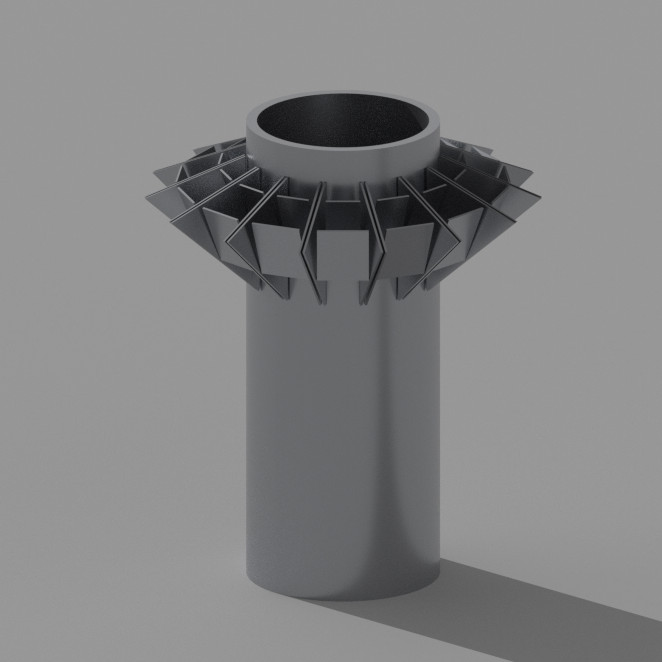
\includegraphics[width=8cm]{media/01_project/render_bin.jpg}\\\vtitle{}}
\subtitle{\vsubtitle{}}
\author{\vauthor{}}
\date{\today}

\maketitle

\addtocontents{toc}{~\hfill\textbf{Seite}\par}

\tableofcontents

\chapter{Einleitung}

    Dieser Projektbericht ist im Rahmen der Cross Innovation Class 2022 entstanden.

\section{Cross Innovation Class}

    Die Cross Innovation Class, kurz CIC, ist eine von der Hamburg Kreativ Gesellschaft organisierte Veranstaltung in Kooperation mit Universitäten und Fachhochschulen des Hamburger Umlands.
    Idee der CIC ist es Studierende verschiedener Fachrichtungen unterschiedlicher Universitäten ein Semester lang in interdisziplinären Teams an Projekten zusammenarbeiten.

    Teilnehmen konnten Studierende des Studiengangs Stadtplanung der Hafencity Universität Hamburg, der Studiengänge Produkt- und Interior-Designer der Akademie Mode \& Design des Standorts Hamburg und der Studiengänge Informatik, Technische Informatik, Wirtschaftsinformatik, Smart Technology und IT-Ingenieurwesen der Fachhochschule Wedel.

    Die Cross Innovation Class lief dabei dieses Jahr unter dem Thema Resilient Cities. In Bezug auf dieses Oberthema wurden fünf Partnerunternehmen ausgesucht, die jeweils eine Fragestellung mit in die CIC gebracht haben.


    \vspace{1em}
    \framebox[\textwidth]{
        \begin{minipage}{\textwidth-1em}
            \vspace{.4em}
            \textbf{Resilient Cities}
            \\ \\
            Resilienz, ein wichtiger Faktor in vielen Lebensbereichen.
            Ein Attribut das Anpassungsfähigkeit und einen standhaften Umgang mit Krisen beschreibt.
            Neben persönlicher und ökonomischer Resilienz übernimmt Resilienz auch eine immer wichtiger werdende Rolle im Blick auf Gemeinden und Städte.
            Vorallem im Bezug auf Extremwetterereignisse und dem immer weiter voranschreitenden Klimawandel braucht es neue Ideen und Konzepte.
            \\ \\
            Daher gibt es viele Bestrebungen auf globaler, europäischer und nationaler Ebene dieses Thema voranzubringen. Eine Institution ist der Urban Resilience Club, der Urbane Resilienz wie folgt definiert:
            \\
            \enquote{Urban Resilience - The measurable ability of any urban system, with its inhabitants, to maintain continuity through all shocks and stresses, while positively adapting and transforming toward sustainability.}\footnote{\url{https://urbanresiliencehub.org/what-is-urban-resilience/}}
            \\
        \end{minipage}
    }
    \vspace{1em}
    
    Partner dieses Jahr waren die Stadt Frankfurt mit der Stabsstelle Digitalisierung, die ACO Gruppe, Hamburg Marketing, Hamburg Institute for Innovation, Climate Protection and Circular Economy (HiiCCE) und das Wald Stadt Labor Iserlohn. \\

    Fünf Teams, jeweils bestehend aus Studierenden jeder Universität und einem Praxispartner durchliefen über knapp 12 Wochen ein Design Thinking Prozess, der 

    \begin{figure}[h]
        \begin{center}
            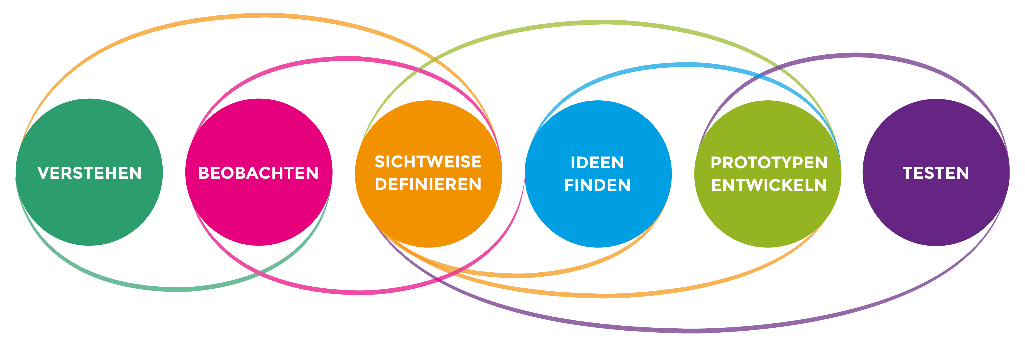
\includegraphics[width=12cm]{media/00_introduction/design_thinking_2.png}
        \end{center}
        \caption{Der Design-Thinking-Prozess\protect\footnote{Quelle: Design Thinking Workshop CrossInnovationClass}}
        \label{fig:dt_2}
    \end{figure}

    \begin{figure}[h]
        \begin{center}
            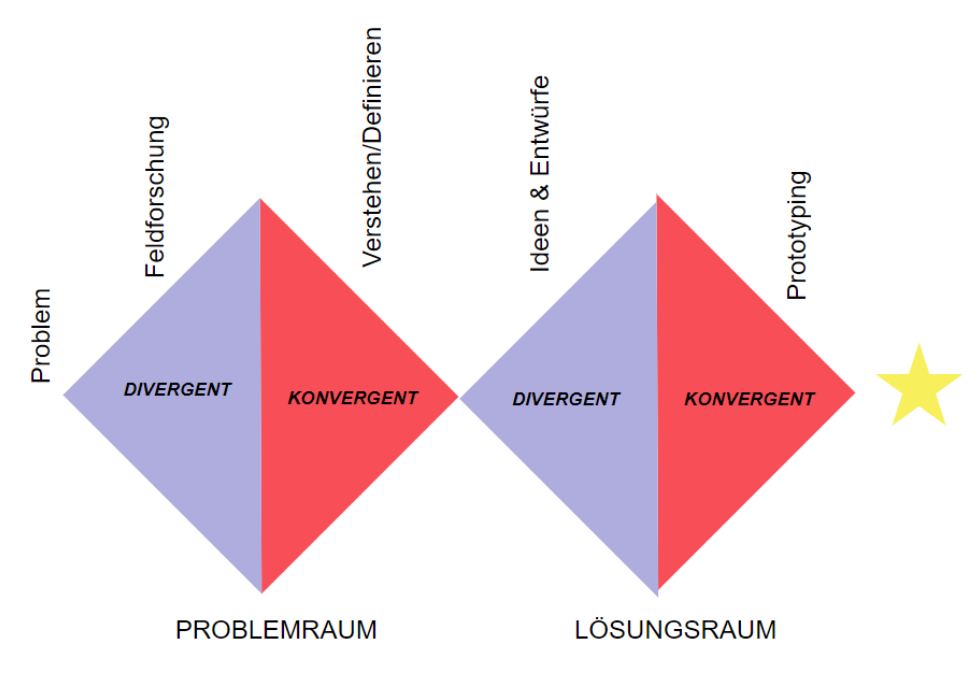
\includegraphics[width=12cm]{media/00_introduction/design_thinking_1.png}
        \end{center}
        \caption{Denkmodell \enquote{Double Diamond}\protect\footnotemark[\value{footnote}]}
        \label{fig:dt_1}
    \end{figure}
    

    \vspace{1em}
    \framebox[\textwidth]{
        \begin{minipage}{\textwidth-1em}
            \vspace{.4em}
            \textbf{Design Thinking}
            \\ \\
            Design Thinking ist ein Prozess zur Ideenfindung und -entwicklung.
            Dabei steht der Mensch im Mittelpunkt der mit einem Problem konfrontiert ist.
            
            Abbildung\,\ref{fig:dt_2} Zeigt die sechs Phasen, sowie die 

            In vielen Veranstaltungen der CIC ist uns der \enquote{Double Diamond} (Abbildung\,\ref{fig:dt_1}) begegnet, denn auch der Ablauf der Cross wurde in einem solchen Rahmen strukturiert.
            \vspace{.4em}
        \end{minipage}
    }
    \vspace{1em}

    Dieses Format stellt im Vergleich zu den sonst eher theoretischeren oder fachspezifischeren Veranstaltungen eine willkommene Ergänzung da.

    \subsection{Ablauf der CIC}

        Das Projekt wurde in drei große Phasen eingeteilt, Konzept, Entwurf und Prototyping.

        Neben einem KickOff zu Beginn gab es am Ende jeder Phase eine Feedback Runde mit der gesamten Class.
        
        In der KickOff Veranstaltung haben sich die Praxispartner und ihre Fragestellung vorgestellt und wir haben unser Team kennengelernt.



        Zusätzlich wurde allen Interessierten vor der Abschlussveranstaltung ein sehr lehrreiches Pitch-Training angeboten.

        Wie sind die Teams enstanden, was hatten wir für (Regel)Termine, wie viel Zeit hatten wir für die unterschiedlichen Aufgaben, etc.
        Skizzierung des CiC-Prozesse.

    \subsubsection{Projektphasen}

        \begin{center}
            \begin{tabular}{ |c|c|c| } 
                \hline
                \printdate{2022-04-08} & Kick-Off \\
                \hline
                \hline
                \printdate{2022-04-11} - \printdate{2022-04-21} & Analyse \& Konzept Phase \\ 
                \hline
                \printdate{2022-04-25} - \printdate{2022-05-06} & Entwurfsphase \\
                \hline
                \printdate{2022-05-09} - \printdate{2022-06-23} & Prototyping \& Modellbau Phase \\
                \hline                
                \hline
                \printdate{2022-06-30} & Abschlussveranstaltung \\
                \hline
            \end{tabular}
        \end{center}


\section{Team Frankfurt}

        
        Unser Team 

        \begin{figure}[h]
            \begin{center}
                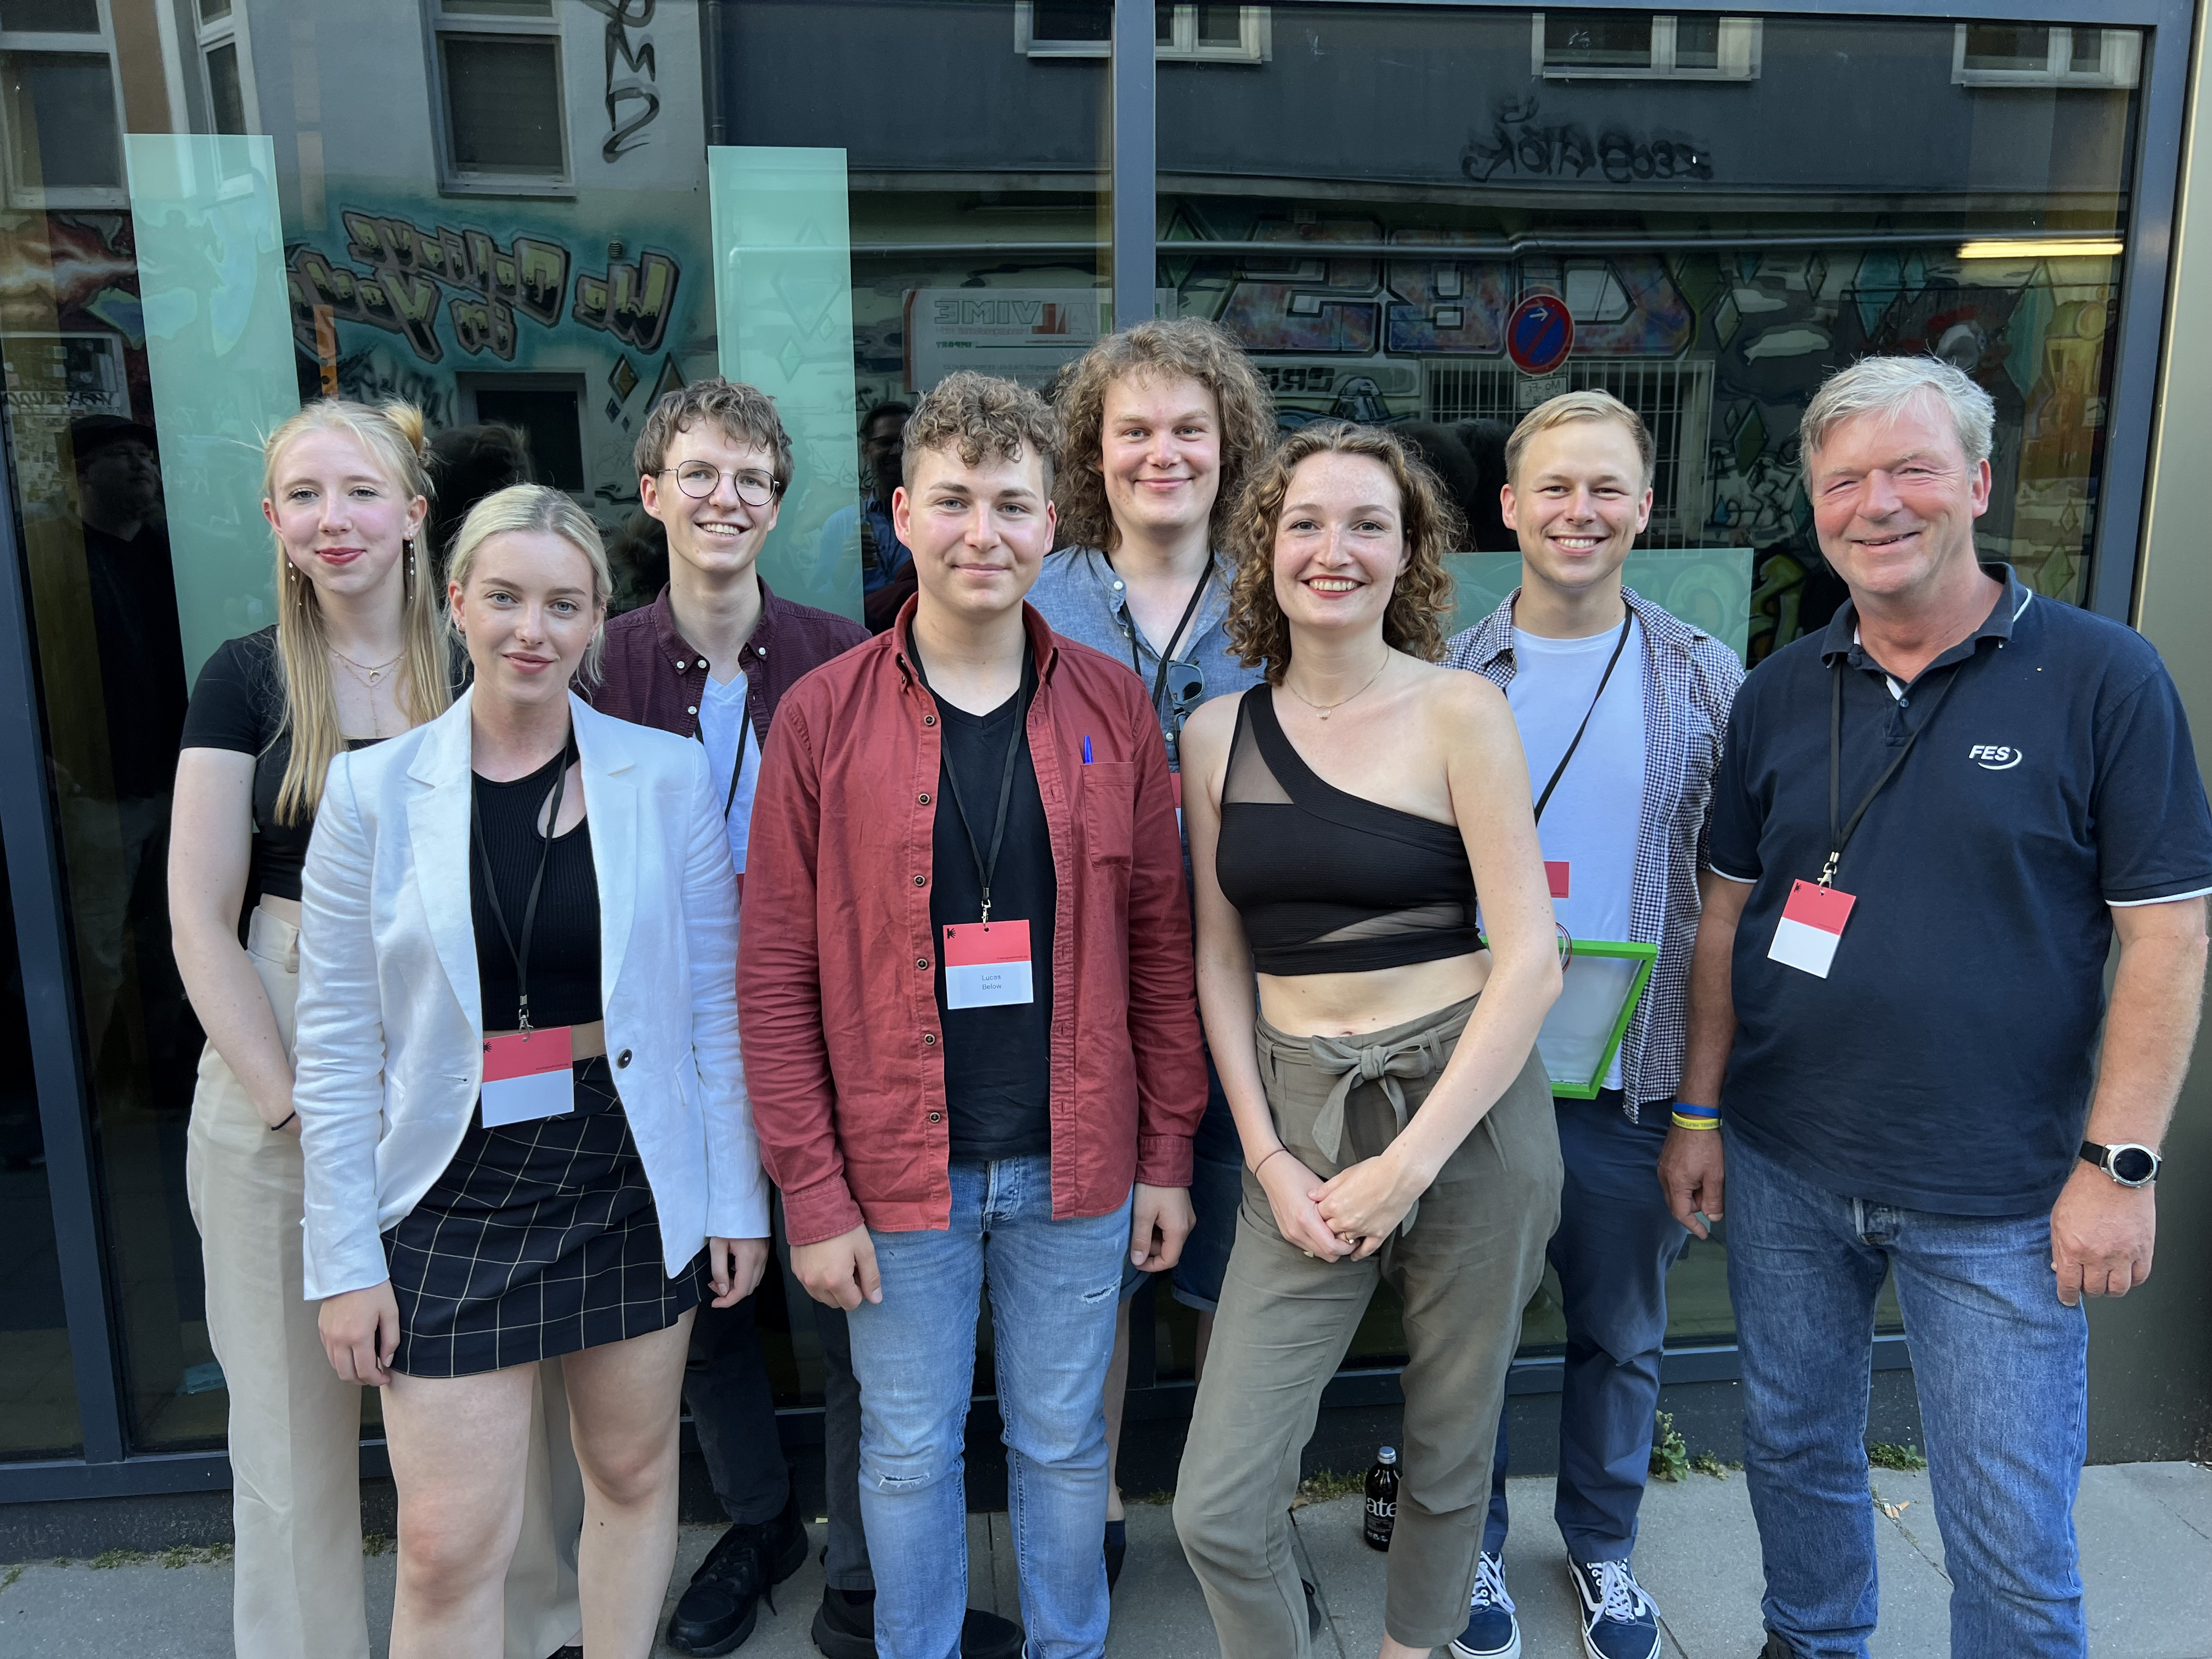
\includegraphics[width=12cm]{media/00_introduction/pic_team-FFM.jpg}
            \end{center}
            \caption[CIC Team Stadt Frankfurt]{CIC Team Stadt Frankfurt \par \small v.l.n.r.: Maybritt Braun (AMD), Annika Fröhlich (AMD), Robin von Berg (FHW), Lucas Below (AMD), Sven Hülsen (FHW), Celina Krug (HCU), Moritz Hillen (HCU), Jochen Schmitz (FES). Abwesend: Florian Bucher (HCU), Mechthild Schulze \& Karina Mombauer             (Stadt Frankfurt Stabstelle Digitalisierung)}
            \label{fig:team_frankfurt}
        \end{figure}

\section{Stadt Frankfurt - Stabstelle Digitalisierung}


    Beschreibung des Industriepartners


\section{Frankfurter Entsorgungs- und Service GmbH (FES)}

    Beschreibung des Industriepartners

\chapter{Projektfindung}\label{chp:projektfindung}

    Zu Beginn des Projekts wurden wir von unserem Praxispartner mit drei Fragestellungen konfrontiert, unter denen wir eine wählen konnten:

    \vspace{1em}
    \begin{tabular}{ l|p{13.5cm} }
        \quad & Wie lässt sich der Verkehr für Einkäufe und Lieferungen reduzieren, um die Schadstoffbelastungen in der Luft zu minimieren?
    \end{tabular}
    \\[1em]
    \begin{tabular}{ l|p{13.5cm} }
        \quad & Wie lässt sich die Müllentsorgung in der Innenstadt und in den Grünflächen optimieren (z.B. Roboter, automatische Mülltrennung, Füllstandsensoren etc.)?
    \end{tabular}
    \\[1em]
    \begin{tabular}{ l|p{13.5cm} }
        \quad & Wie lässt sich Informations- und Kommunikationstechnik (IKT) (Rechenzentren, WLAN, Breitband) für eine umwelt- und ressourcenschonende Stadtgestaltung (z.B. Abwärme der Rechenzentren) nutzen? 
    \end{tabular}
    \vspace{1em}

    Im Anschluss der KickOff-Veranstaltung haben wir uns für die zweite Frage die das Thema Müllentsorgung thematisiert entschieden, da wir dabei die größten Freiheiten bei der Gestaltung des Prototyps gesehen haben und Lust hatten uns mit der Problematik auseinander zu setzen.

    So haben wir in den kommenden Wochen Interviews mit unseren Praxispartnern geführt, nach schon existierende Maßnahmen und der aktuellen Lage vor Ort, sowie nach psychologischen Ursachen recherchiert.
    
    So konnten wir unseren Problemraum immer größer gestalten, bis wir beim CIC Workshop vier Ideen vorgestellt haben. (\href{run:attachments/Frankfurt_Ideen_CIC.pdf}{\textbf{PDF der Präsentation}})

    \begin{figure}[h]
        \begin{center}
            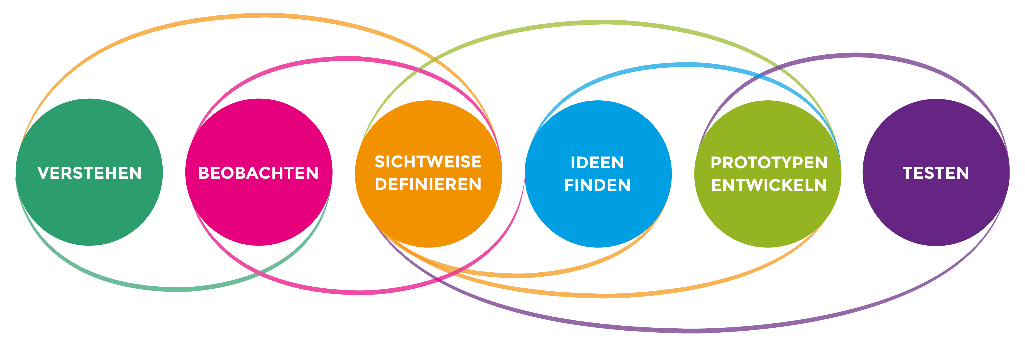
\includegraphics[width=11cm]{media/00_introduction/design_thinking_2.png}
        \end{center}
        \caption{Der Design-Thinking-Prozess\protect\footnote{Quelle: Design Thinking Workshop CrossInnovationClass}}
        \label{fig:dt_2}
    \end{figure}

    \vspace{1em}
    \framebox[\textwidth]{
        \begin{minipage}{\textwidth-1em}
            \vspace{.4em}
            \textbf{Design Thinking}
            \\[1em]            
            Design Thinking ist ein Prozess zur Ideenfindung und -entwicklung.
            Dabei steht der Mensch im Mittelpunkt der mit einem Problem konfrontiert ist.
            
            Abbildung\,\ref{fig:dt_2} zeigt die sechs Phasen die im Prozess durchlaufen werden und visualisiert den iterativen Ansatz, das mehrmalige durchlaufen in unterschiedlichen Kreisen im Laufe des Prozess.\\

            In vielen Veranstaltungen der CIC ist uns besonders das Modell des \enquote{Double Diamonds} (Abbildung\,\ref{fig:dt_1}) begegnet, da der Ablauf der Cross in einem solchen Rahmen strukturiert wurde.
            Anhand der Fragestellung wird ein breiter Problemraum geöffnet in dem möglichst viel Wissen aus verschiedenen Perspektiven zusammenfließt. Diese Problemdefinition wird nun konkretisiert, um einen Lösungsraum zu öffnen, der Lösungsansätze jeder Art zulässt.
            Anschließend werden auch diese im Team besprochen und am Ende entsteht ein konkreter Prototyp.
            \vspace{.4em}
        \end{minipage}
    }
    \vspace{1em}

    \begin{figure}[h]
        \begin{center}
            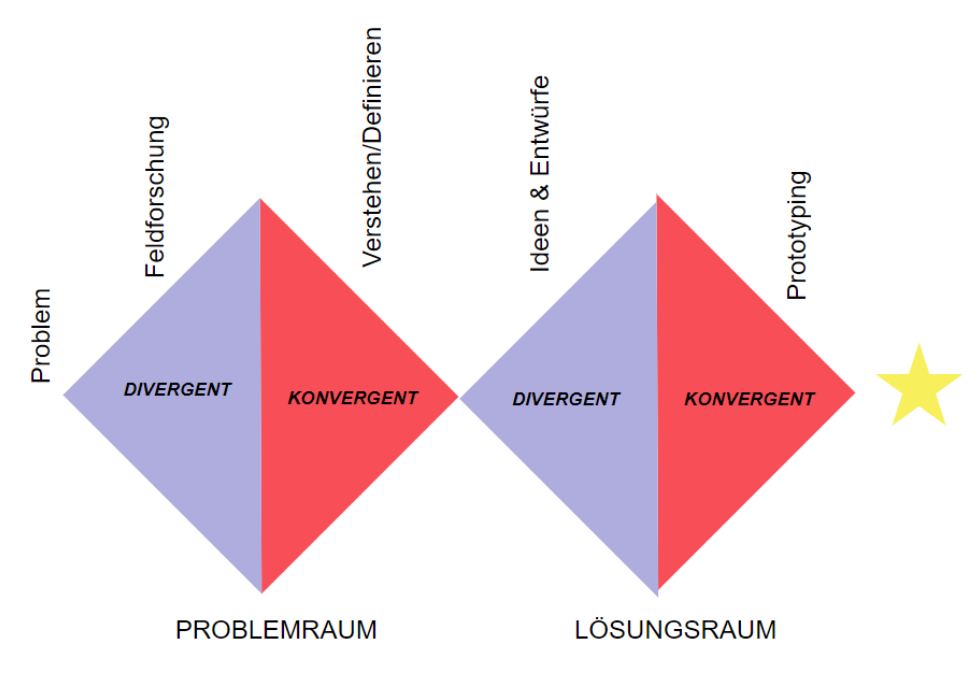
\includegraphics[width=10cm]{media/00_introduction/design_thinking_1.png}
        \end{center}
        \caption{Denkmodell \enquote{Double Diamond}\protect\footnotemark[\value{footnote}]}
        \label{fig:dt_1}
    \end{figure}

    Dabei hatten wir alls Team zwei Favoriten.

    Die Idee, die es nicht geschafft hat, war der sogenannte \enquote{Bar-Bus}.Er sollte ein ausgebauter Bully sein, der verschiedene Konzepte vereint hätte. Darunter fällt ein  als Rutsche umgesetzter Flascheneinwurf, die Möglichkeit den Bus zu beschreiben und bemalen, sowie ein Angebot Snacks in müllfreier Verpackung und Entertainment-Angebote, wie Musik.
    Er sollte eine Anlaufstelle für die Menschen werden, die Aufgrund ihrer Kleidung, ihres Ausshehens oder ihrer finanziellen Mittel oft den Zugang  zu den Frankfurter Clubs verwehrt bekommen.

    Problematisch an der Idee war, dass die Stadt hier als Anbieter von Waren auftritt und ebenfalls die Party-Stimmung nicht mindert, auch wenn dadurch wohlmöglich die aggressive und rücksichtslose Atmosphäre minimiert wird.

    Daher haben wir im weiteren Verlauf unsere zweite Idee, einen interaktiven Mülleimer verfolgt, den wir im nächsten Kapitel ausführlich beschreiben.


\chapter{Projektbeschreibung}

\section{Grundlegende Konzepte}
    
    Die Idee des interaktiven Mülleimers (anfänglich als \enquote{Party-Bin} bezeichnet) soll das Problem lösen, dass manche Feiernden den Weg zum Mülleimer nicht finden, sodass, vorallem in der Corona-Zeit, die Parks und Plätze sowie das Main-Ufer Samstag und Sonntag Morgens extrem vermüllt waren.

    Den ersten psychologischen Effekt den wir anwenden wollten, ist der Aspekt der Gamification. Wir wollten die Menschen dafür belohnen, dass sie ihren Müll fachgerecht im Mülleimer entsorgt haben. Dabei wollten wir erreichen dass der Mülleimer selbst auf den Mülleinwurf reagiert. Ebenfalls wichtig war uns, dass es einfach und intuitiv bleibt, keine App, kein komplexes Konzept, ein einfaches Feedback, das jeden Mülleinwurf belohnt.

    Die möglichen Feedbackansätze bestanden in unseren Überlegungen aus einem auditiven Feedback, bspw. einem Geräusch, einer menschlichen Stimme oder  Musik oder einem visuellem Feedback, welches per direkter oder indirekter Beleuchtung zu realisieren wäre.

    \begin{figure}[H]
        \centering
        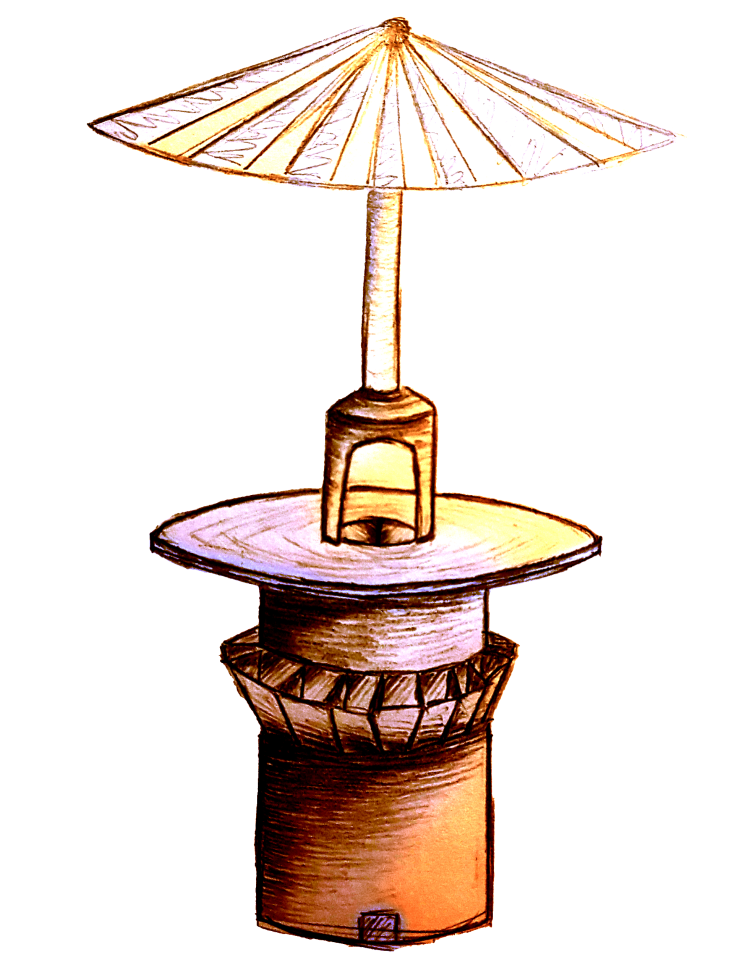
\includegraphics[width=5cm]{media/01_project/sketch_standing_table_bin.png}
        \caption{Konzept eines Tischmülleimers, der einige der Konzepte umsetzt.}
        \label{fig:standing_desk_bin_1}
    \end{figure}

    In unserem ersten Ansatz haben wir uns auf Musik fokussiert, die Möglichkeit belohnt zu werden in dem man beim Einwurf für ein nächstes Lied abstimmen kann, oder als Ansatz um die Feiernden in die Nähe der Mülleimer zu bekommen, eine Abstimmung an der jeder Mülleimer ein Lied repräsentiert und misst, wieviele Menschen um ihn herrum stehen. Bei diesem Ansatz konnten wir ein paar große Risiken nicht ausmerzen, einerseits ebenfalls das Argument, dass diese Mülleimer die Partystimmung stärker anheizen könnten, andererseits das Thema der Rechte an der Musik.
    Ein Beispielentwurf ist in der Skizze\,\ref{fig:standing_desk_bin_1} zu sehen.\\

    Der zweite Ansatz basierte daher nun auf Licht.
    Ein erster Entwurf des ganzen ist die Skizze\,\ref{fig:light_bin_1}.
    Dieser Mülleimer reagiert beim Einwurf von Müll mit einer kleinen \enquote{Lichtshow}.\\

    In beiden Skizzen (\ref{fig:standing_desk_bin_1} \& \ref{fig:light_bin_1}) zu entdecken ist ein Pfandring. Da unsere Recherchen ergeben haben, dass ein großer Teil des anfallenden Mülls auf Flaschen zurückzuführen ist und wir von Jochen Schmitz eine positive Erfahrung mit einem eingesetzten \enquote{Pfandregal} geschildert bekommen haben, wollten wir unbedingt Flaschenablagemöglichkeiten in unser Design integrieren.
    Eine Übersicht der In der CIC präsentierten Ideen: (\href{run:attachments/Frankfurt_Entwürfe_CIC.pdf}{\textbf{PDF der Präsentation}})

    \begin{figure}[H]
        \centering
        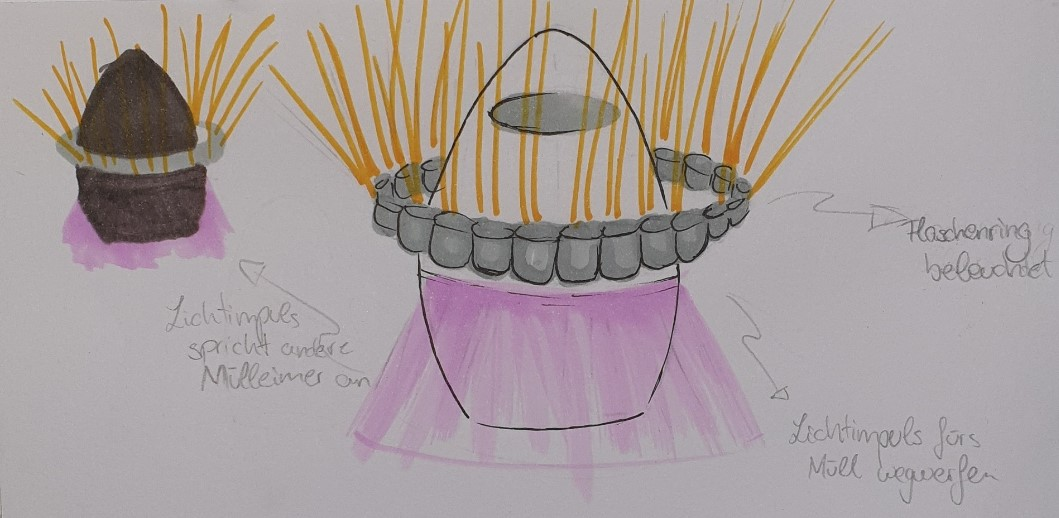
\includegraphics[width=10cm]{media/01_project/sketch_party_bin.jpg}
        \caption{Konzept eines Tischmülleimers, der einige der Konzepte umsetzt.}
        \label{fig:light_bin_1}
    \end{figure}

    Ausgehend aus diesen Überlegungen haben wir letztendlich ein finalen Entwurf zusammengestellt. Dieser ist minimalistischer im Design und in der Art der Beleuchtung, um sich besser ins Stadtbild einzufügen.
    An unserem Design optisch am auffälligsten ist der Flaschenring.

    \begin{figure}[H]
        \centering
        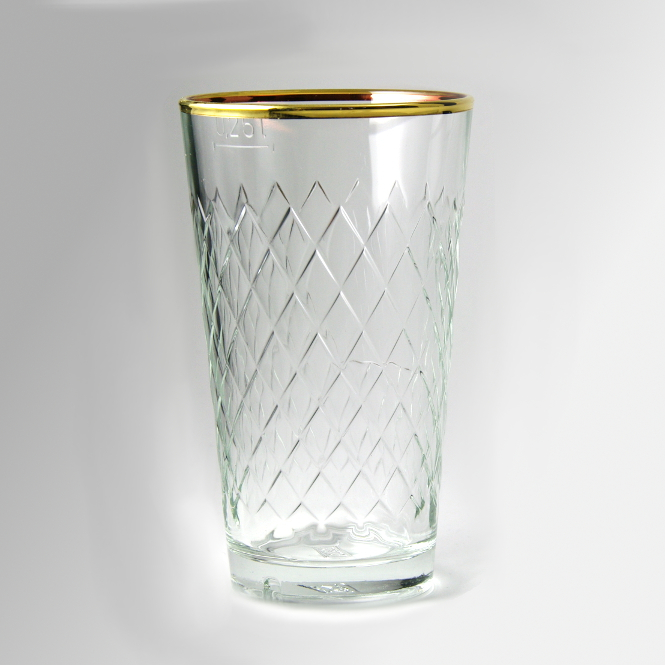
\includegraphics[width=5cm]{media/01_project/picture_geripptes.jpg}
        \caption{Das \enquote{Gerippte}.}
        \label{fig:picture_gerippte}
    \end{figure}

    Das Design entleiht sich dabei die Rauten am Rand des Zylinders unterhalb des Flaschenrings vom Frankfurter Gerripten, einem Apfelweinglas, das sich hoher lokaler Beliebtheit erfreut. Ein Beispielglas ist in der Abbildung\,\ref{fig:picture_gerippte} zu sehen. Neben der passenden Integration in unser Flaschenring wollen wir damit eine höhere Identifikation erzeugen.
    Ebenfalls konnten wir die Rautenstruktur verwenden um unsere Beleuchtung dort einzubauen, sodass sich das Modell selbst beleuchten kann und das Licht durch die Reflexion diffuser wird.
    
    \begin{figure}[H]
        \centering
        \begin{subfigure}[b]{\textwidth}
            \centering
            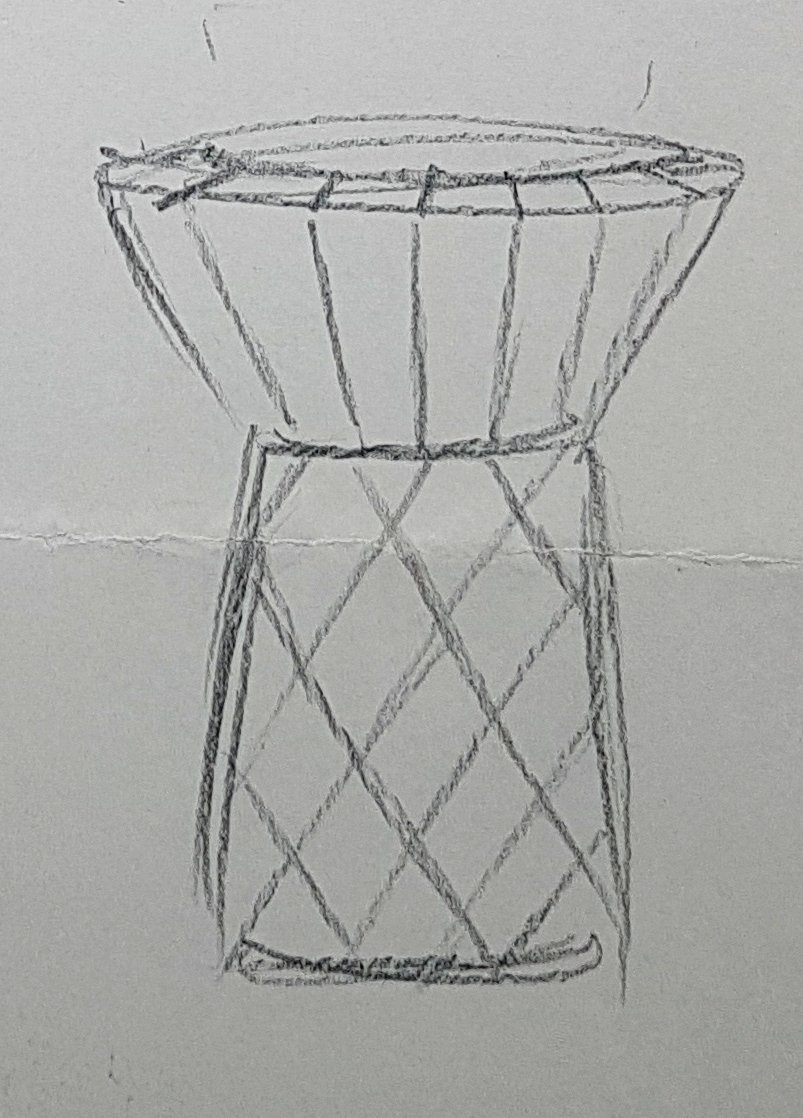
\includegraphics[width=0.32\linewidth]{media/01_project/pencil_sketch_bin_2.jpg}
            \hspace{1cm}
            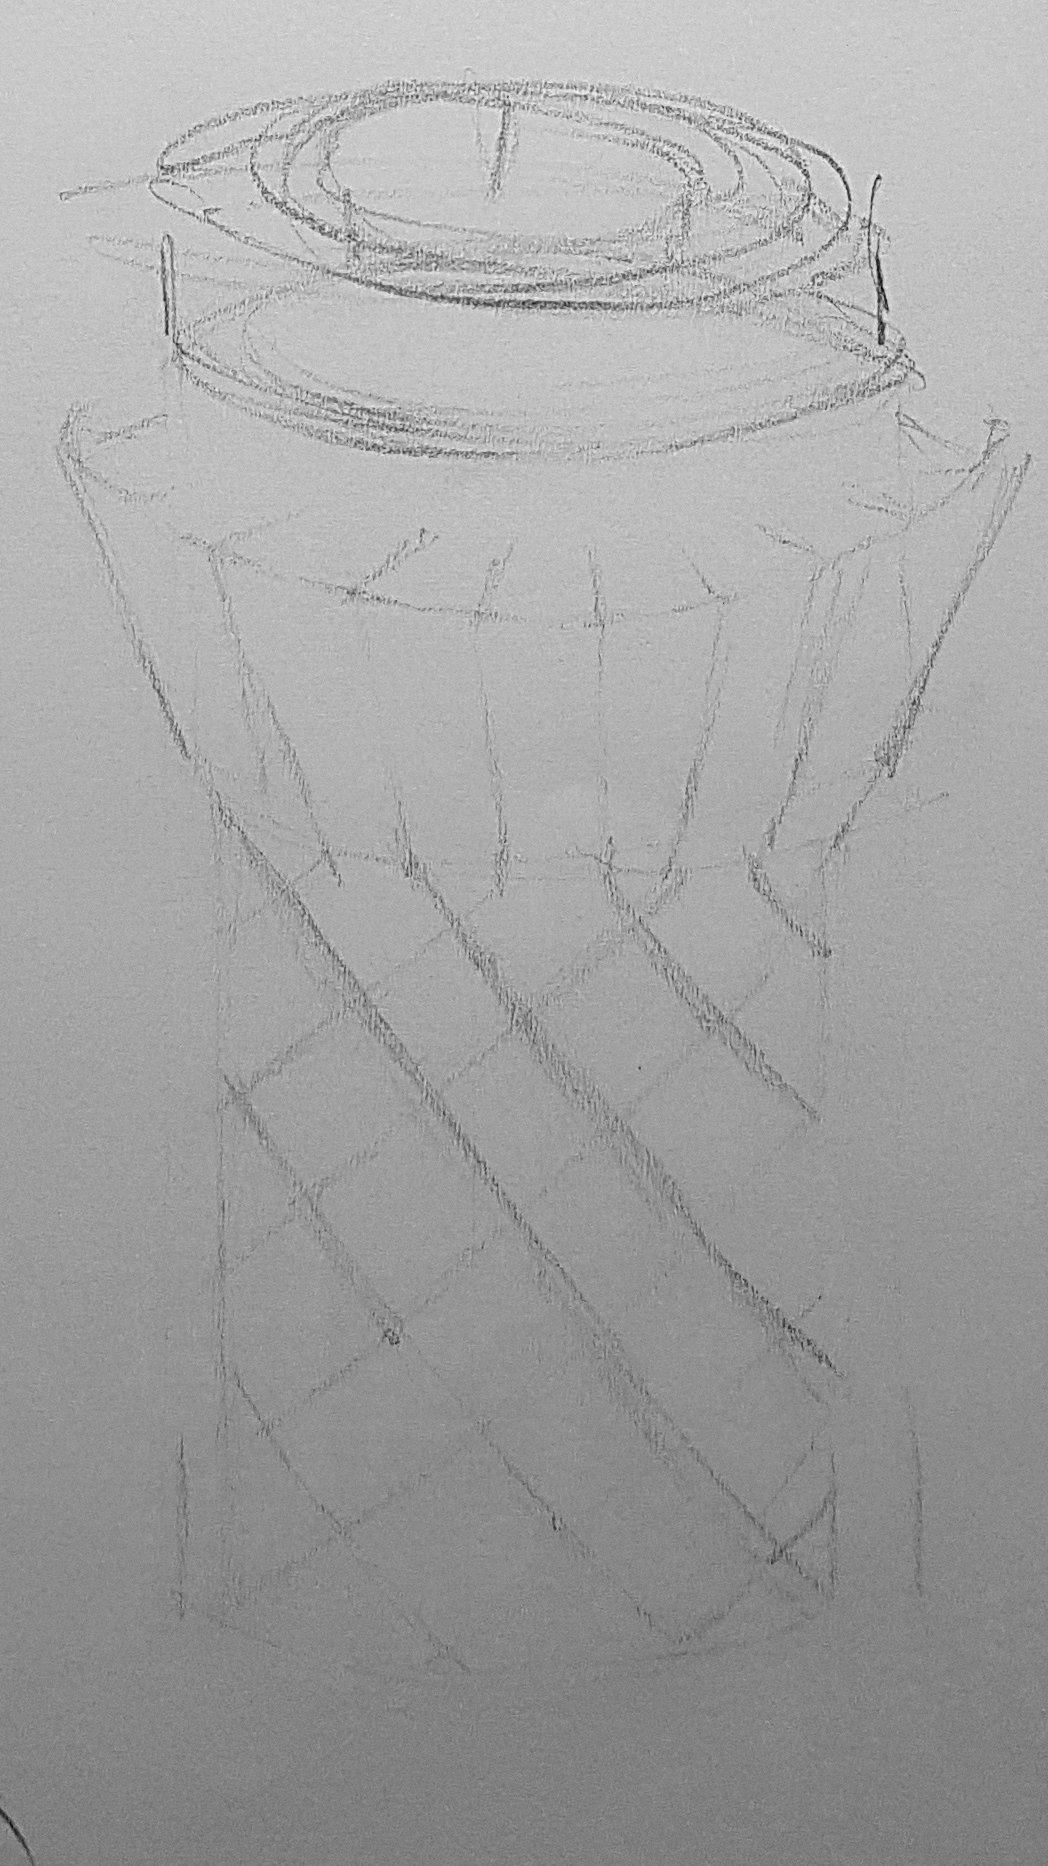
\includegraphics[width=0.32\linewidth]{media/01_project/pencil_sketch_bin_3.jpg}
        \end{subfigure}
        \caption{Skizzen des Entwurfs mit Rautenmuster}
        \label{fig:pencil_bin_2}
    \end{figure}

    Ein weiterer Vorteil des visuellen Ansatzes ist die stärkere Präsenz im Unterbewusstsein der Feiernden. Wir Menschen reagieren Abseits unseres Fokuspunktes (der Punkt den wir aktuell betrachten) instinktiv auf Kontraste und Bewegungen. Ein sich im Blickfeld befindender Mülleimer der dezent aufleuchtet wird unterbewusst wahrgenommen.

    \begin{figure}[H]
        \begin{center}
            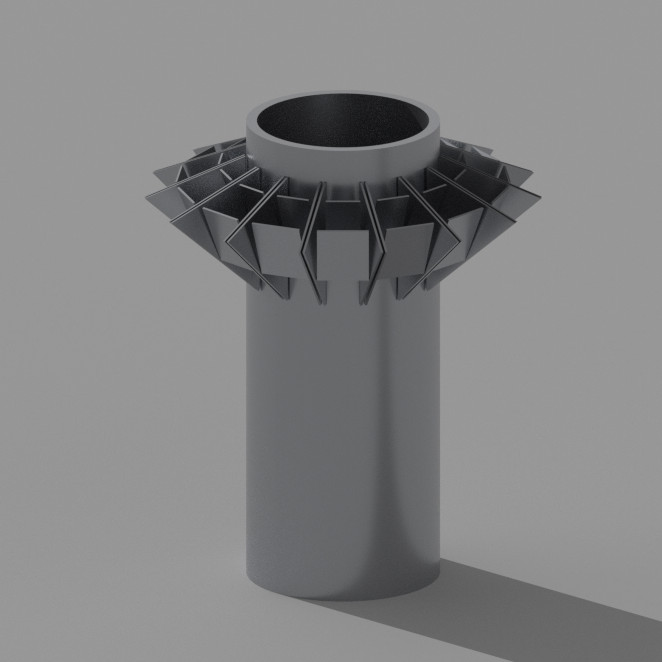
\includegraphics[width=7cm]{media/01_project/render_bin.jpg}
        \end{center}
        \caption{Render des Entwurfs mit Fokus auf den Flaschenring}
        \label{fig:pencil_bin_3}
    \end{figure}

\section{Funkionen}\label{cpt:funktionen}

    Das Modell besitzt drei Grundfunktionen:

    \subsubsection{Visuelles Feedback bei Mülleinwurf}
        
        Wirft jemand Müll in den Mülleimer, so leuchten die Rauten in einer kurzen Animation auf.
        Wird in einem bestimmten Intervall mehrmals Müll eingeworfen, so wird die Animation intensiver. Damit haben wir eine weitere Motivation Müll zu sammeln, sowie ein dezentes Auftreten am Tag, wenn er nur sporadisch verwendet wird.
      

    \subsubsection{Beleuchtung von Flaschen im Flaschenring}

        Als weitere Funktion sollen in den Flaschenring gestellte Flaschen von von unten beleuchtet werden. Auch hier erhält die Person ein direktes Feedback, das optisch zusätzlich sehr ansprechend aussieht.
        Wird ein gesamter Flaschenring verwendet, so spielt der Mülleimer ebenfalls eine Animation.


    \subsubsection{Ein mehrere Mülleimer übergreifender Lichtimpuls}

        In speziellen Fällen, beispielsweise bei zehn Mülleinwürfen in kurzer Zeitspanne oder bei einem gefüllten Flaschenring, soll die Animation als Impulswelle an benachbarte Mülleimer weitergeleitet werden.
        Dies dient als weiterer Ansporn, der einen möglichen Wettbewerbsehrgeiz erzeugt, falls mehrere Gruppen an Feiernden anwesend sind.
        Allgemein Wichtig in der Realisation ist hier, dass die Animationen einen Weg zwischen nicht zu auffällig, aber wahrnehmbar finden.
        Wir haben diesen Grad immer als Lagerfeuerstimmung bezeichnet.

\chapter{Aufgaben}

\section{Aufgabenverteilung}

Darstellung der Aufgabenverteilung innerhalb des Teams, ggf. durch
eine Tabelle

Verweise auf das Projekt-Repository in dem weitere
Projekt-Artefakte zu finden sind (s.u.).
\chapter{Technische Realisation}

\section{Aufgabenbereiche}

    % Welche Komponenten müssen technisch realisiert werden? 


    % Siehe Technische Daten

    % Beschreibung der prototypischen Realisierung, Vorgehensweise und
    % Beschreibung einzelner Schritte


    % Beschreibung der prototypischen Realisierung, Vorgehensweise und  Beschreibung einzelner Schritte
    % Verweise auf das Projekt-Repository in dem weitere Projekt-Artefakte zu finden sind (s.u.).






    Die technischen Aspekte des Gerippten lassen sich grob in folgende Teilbereiche aufgliedern:

    \begin{itemize}
        \item Beleuchtung der Tonnenaußenwand inklusive Animation der Lichteffekte sowie Beleuchtung des Flaschenrings
        \item Sensorik zur Detektion von Flaschen im Flaschenring
        \item Detektion von Gegenständen die in den Behälter geworfen werden
        \item Messung des Füllstandes
        \item Verkablung der Sensorik und der LEDs.
        \item Austausch von Informationen zwischen mehreren Endgeräten
        \item Verarbeitung der Sensordaten und Ansteuerung der Beleuchtung
    \end{itemize}

    In den nachfolgenden Kapiteln werden die zur Realisierung der verschiedenen Teilaspekte genutzten Komponenten beschrieben und diskutiert.

\addtocontents{toc}{\protect\setcounter{tocdepth}{1}}

\section{Mikrocontroller}
    \subsection{Diskussion}
        Als zentrale Steuerungskomponente ist die Wahl des Mikrocontrollers von zentraler Bedeutung für die technische Realisierung des Projekts. Die wichtigste Eigenschaft des Mikrocontrollers war in diesem Projekt die generelle Verbreitung des Mikrocontrollers, da die Einarbeitungszeit sehr kurz ist und somit eine große Auswahl von Informationsquellen entscheidende Vorteile bringt. Dadurch stechen zwei Hersteller besonders heraus. Zum einen Arduino, die eine große Auswahl unterschiedlichster Mikrocontroller mit verschiedenstem Funktionsumfang anbieten und zum anderen Espressif, deren ESP32 Mikrocontroller eher als "Alleskönner" bezeichnet werden kann, da er im Vergleich zu den meisten Arduino Modellen wesentlich mehr und bessere Hardware bietet.
        Eine weitere Möglichkeit bietet die Nutzung des Einplatinencomputers Raspberry Pi, der einen weitaus größeren Funktionsumfang und wesentlich mehr Rechenleistung besitzt als ein Mikrocontroller. Die Nachteile des Raspberry Pi liegen in den hohen Anschaffungskosten und dem ebenfalls hohen Stromverbrauch. Im allgemeinen ist ein Raspberry Pi für dieses Projekt überdimensioniert, da ein Großteil des Mehrwertes den dieser gegenüber einem Mikrocontroller bietet in diesem Projekt keine Verwendung fände.\\
        
        Da eine kabellose Kommunikation der Mikrocontroller untereinander realisiert werden soll, ist es essenziell, dass der Mikrocontroller mit einem WiFi oder Bluetooth Modul ausgestattet ist. Der ESP32 bringt beides mit. Arduino bietet ebenfalls einige Modelle an, die mit mindestens einem der Module ausgestattet sind. Insbesondere die Nano 33 Reihe von Arduino bietet Geräte, die für die Verwendung in diesem Projekt die notwendigen Kriterien erfüllen. Hier sind speziell die Modelle Nano 33 BLE und Nano 33 IoT hervorzuheben. Das Modell Nano 33 IoT ist dabei speziell für die Verwendung in Internet of Things Geräten designed und bietet sowohl ein WiFi als auch ein Bluetooth Modul. Das Modell Nano 33 BLE besitzt lediglich ein Bluetooth Modul, dieses ist jedoch mit Bluetooth 5 etwas moderner als die Bluetooth 4.2 Variante, die im Nano 33 IoT Modell verbaut ist. Zudem besitzt das BLE Modell einen leistungsstärkeren Prozessor, der jedoch durch integrierte Energiesparfunktionen mindestens genauso energiesparend ist. Der Energieverbrauch stellt sich für dieses Projekt ebenfalls als wichtiger Faktor heraus, da für eine mögliche Weiterführung des Projekts eine Stromversorgung der Geräte über Solarzellen und Akkus implementierbar sein soll. Die hier diskutierten Vor- und Nachteile der 3 zur Verfügung stehenden Mikrocontrollern wird in Tabelle \ref{tab:compare_mics} nochmals in kürze zusammengefasst.

        \begin{table}[H]
            \caption{Vergleich der Mikrocontroller ESP32, Nano 33 IoT und Nano 33 BLE}
            \centering
            \begin{tabularx}{\textwidth}{  X | X | X  }
                \textbf{Espressif ESP32} & \textbf{Arduino Nano 33 IoT} & \textbf{Arduino Nano 33 BLE}\\ [0.5ex] \hline\hline
                Leistungsstärkster Mikrocontroller &
                Am wenigsten Leistung im Vergleich &
                Leistungsstarker Prozessor\\
                &&\\
                Bluetooth \& WiFi &
                Bluetooth \& WiFi &
                Nur Bluetooth, dafür Bluetooth 5 \\
                &&\\
                Vergleichsweise hoher Stromverbrauch &
                Geringer Stromverbrauch &
                Geringer Stromverbrauch \\
            \end{tabularx}
            \label{tab:compare_mics}
        \end{table}

        Im Kapitel \ref{communications} wird erläutert, dass die Kommunikation über den Bluetooth beziehungsweise Bluetooth Low Energy Standard erfolgen soll. Somit bieten die WiFi Module, die der ESP32 und der Nano 33 IoT Mikrocontroller mitbringen keine weiteren Vorteile gegenüber dem Nano 33 BLE Mikrocontroller. Da dieser außerdem einen sehr geringen Stromverbrauch im Verhältnis zu seiner Leistungsfähigkeit aufweist, wurde dieser für die Verwendung in diesem Projekt ausgewählt.


    \subsection{Platform}

        Wie in der Arduino Welt üblich programmieren wir in der systemnahen Sprache C++.
        Allerdings haben wir uns


\section{Beleuchtung}
    \subsection{Diskussion}

        Um die Flaschen des Flaschenrings und die Rauten zu beleuchten benötigen wir LEDs. Es eröffnet sich herbei ein großer Raum von Optionen. LEDs sind zu unterscheiden in Größe und Form, in Helligkeit und der Art der Ansteuerung und zwischen RGB- und RGBW-LEDS.
        Eine der Kategorien konnten wir mit dem Rat von Prof. Hoffmann und Simon zu Beginn klären. Um die Menge der benötigten LEDs individuell über ein Arduino ansteuern zu können, benötigen wir LEDs mit einem integriertem Driver-Chip. NeoPixel von Adafruit, oder die vielen äquivalente Optionen auf dem Markt ermöglichen diese Funktionalität in dem sie als 24 oder 32 Bit Shift-Register agieren. Dabei wird die Farbintensität jeder der drei oder vier Farben (RGB oder RGBW) als ein 8-Bit Wert angegeben und von LED zu LED weitergeleitet.
        Wird ein RESET-Signal gesendet, wird der zuletzt gespeicherte Wert angezeigt.

        Weitere Überlegungen mussten wir uns besonders hinsichtlich der Größe und Form machen. Für die Animationen der Tonne wollten wir jede Raute an den oberen Kanten, dessen Längen jeweils ca. 10cm betragen, mit LEDs bestücken. Hierfür haben sich LED-Strips angeboten, wobei wir möglichst schmale benötigen, damit sie, wenn eine Person den Mülleimer von oben anguckt, in der Rautenstruktur verschwinden. Als alternativen Ansatz hatten wir vorher überlegt die Rauten mit einzelnen LEDs zu beleuchten, doch durch den enormen Aufwand der Verkabelung haben wir diesen Ansatz im Laufe der Entwurfsphase wieder verworfen.

        Für die LEDs des Flaschenrings wiederum haben wir vorallem eine weitere Anforderung: Die Helligkeit. Dadurch dass das Licht durch die Flaschen gefiltert wird, müssen wir sichergehen, dass die Lichtintensität hoch genug ist. Bei der Recherche haben wir zwei Optionen gefunden.
        Einerseits ebenfalls die NeoPixel, hier als einzelne LEDS im RGBW Format um eine höhere Helligkeit zu erzielen, andererseits der \enquote{große Bruder}, die Adafruit NeoPixel Pixies. Diese LEDs laufen statt mit 0.2 Watt mit 3 Watt, ein extremer Unterschied, aber dadurch, dass wir 15 Flaschenringfächer haben, mussten wir uns aus Budgetgründen für jeweils zwei LEDs der kleineren Variante entschieden, die mit den Breakoutboards bei 75ct/Stück liegen während sich die Pixies bei 14.95€/Stück außerhalb jedes Rahmens befinden. Ein weiterer wichtiger Faktor den man hätte beleuchten müssen ist die Hitzeentwicklung der großen LEDs, doch so mussten wir nicht in die Details eintauschen.


    \subsection{Implementation}

        \subsubsection{Hardware}

            Wir haben uns bei der Rautenbeleuchtung für 7 Meter Adafruit Mini Skinny NeoPixel Strips entschieden die mit 30 RGB LEDs pro Meter bestückt sind. So konnten wir den Strip in jeweils 20cm Segmenten unterteilen und jede Raute mit insgesamt 6 LEDs beleuchten.
            Der Strip ist mit 1 Ampere Verbrauch pro Meter angegeben, was die Wahl des 10 Ampere Netzteils begründet.
            Die Strip-Segmenten haben wir dann wieder verbunden, in dem wir die drei Kontakte per Kabel an das nächste Segmenten weitergeleitet haben. Die Abstände zwischen den Strips und damit die Kabellängen sind abhängig von der Position am Modell.
            Diese Aufteilung wird in Abbildung\,\ref{fig:led_wiring_rhombus} skizziert.

            \begin{figure}[H]
                \begin{center}
                    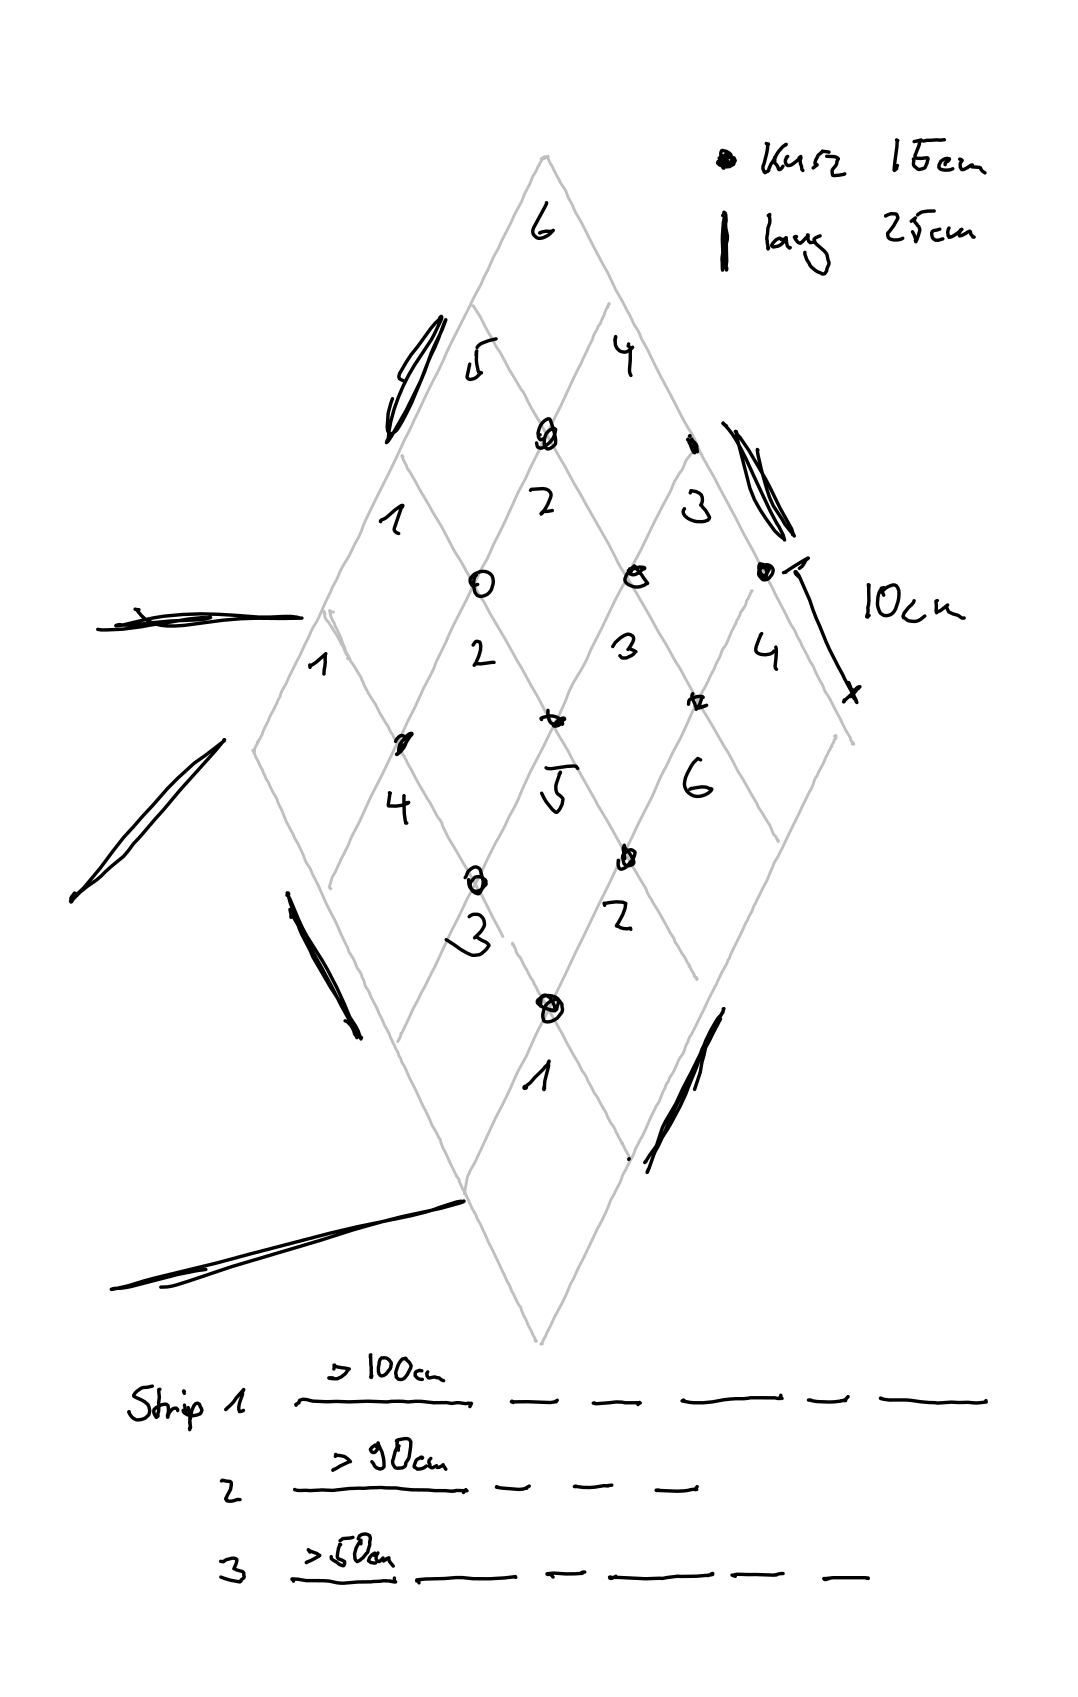
\includegraphics[width=10cm]{media/03_technical_implementation/leds_3.png}
                \end{center}
                \caption{Anordnung der LED-Strips in der Raute am Modell}
                \label{fig:led_wiring_rhombus}
            \end{figure}
            
            Dort zu erkennen ist, dass wir nur ein Teil der Rauten beleuchtet haben, da es uns an LED-Strips fehlte. Eine aus Rauten bestehende große Raute, die wir aus drei Kabel-Strip-Strängen zusammensetzen.
            So laufen am Ende drei Stecker zum Arduino.\\

            \begin{figure}[H]
                \begin{subfigure}[b]{0.5\textwidth}
                    \centering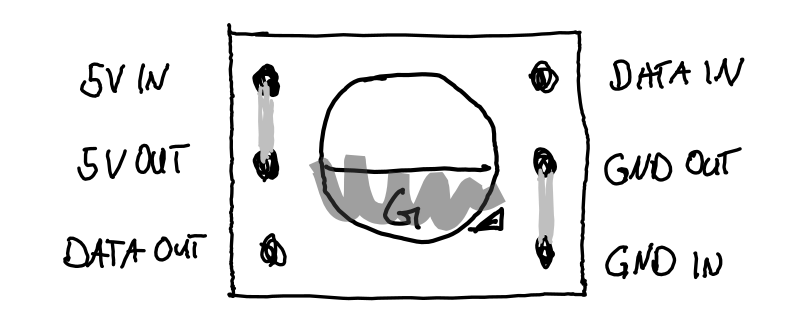
\includegraphics[width=\textwidth]{media/03_technical_implementation/leds_2.png}
                    \caption{Pin-Belegung auf den verwendeten 6-Pin BreakOut-Boards für unsere NeoPixel SK6812RGBW. Gezogene Lötbrücken sind in grau eingezeichnet.}
                    \label{fig:pins_neopixel}
                  \end{subfigure}\quad
                  \begin{subfigure}[b]{0.5\textwidth}
                    \centering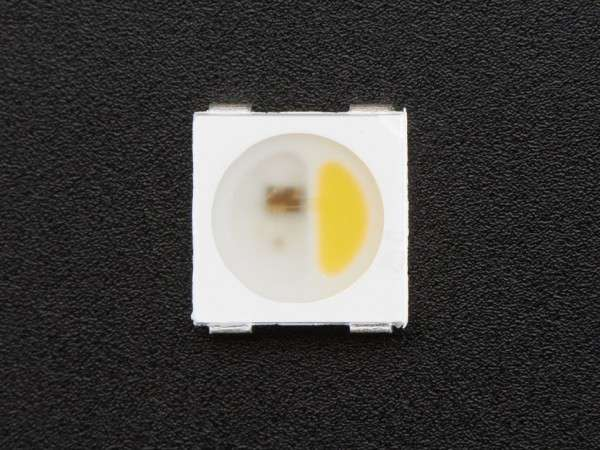
\includegraphics[width=0.7\textwidth]{media/03_technical_implementation/picture_neopixel.jpg}
                    \caption{NeoPixel RGBW LED SK6812RGBW}
                    \label{fig:picture_neopixel}
                  \end{subfigure}
            \end{figure}

            \begin{figure}[H]
                \begin{center}
                    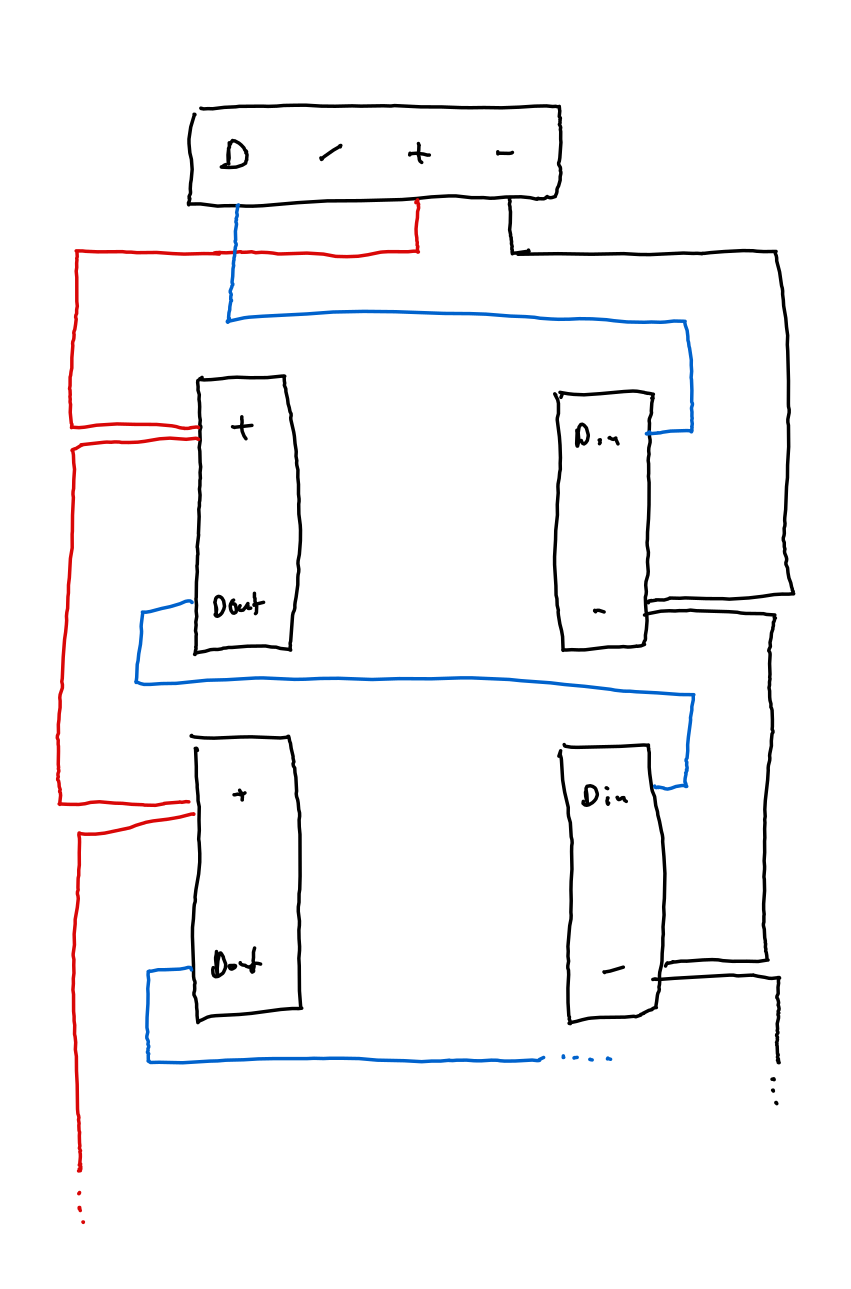
\includegraphics[width=7cm]{media/03_technical_implementation/leds_1.png}
                \end{center}
                \caption{Auszug eines Kabelbaums für die LEDs des Flaschenrings.}
                \label{fig:led_wiring_1}
            \end{figure}
      
            Für die Flaschenring LEDs haben wir Breakoutboards beschafft, auf die wir die LEDs gelötet haben. Diese Boards haben 6 Pins, während die LEDs 4 Pins haben. In der Skizze\,\ref{fig:pins_neopixel} haben wir gezeigt wie wir diese zwei Extra-Pins dafür verwenden, über Lötbrücken Strom und Ground im Kabelbaum an die nächsten LEDs weiterzuleiten. Zwei dieser Kabelbäume hat vorallem Moritz aus der HCU gebaut, wohlmöglich eine der aufwendigsten Unterfange unseres Projekts. Den Aufbau eine solchen Kabelbaums ist in Abbildung\,\ref{fig:led_wiring_1} gezeigt.


            
        \subsubsection{Software}

            Softwareseitig bieten die Neopixel eine sehr gute Integration im Arduino Universum mit der Bibliothek \href{https://github.com/adafruit/Adafruit_NeoPixel}{\enquote{Adafruit\_NeoPixel}}.
            Jeder LED-Strang benötigt nur ein Digital-Pin als Datenleitung.
            In der Initialisierung werden Pin-Nummer, Anzahl der hintereinander geschalteten LEDs und der Anordnung der Farbwerte in den Chips benötigt. Für die LEDs des Flaschenrings ist das GRBW für die LED-Strips GRB.
            Ab diesem Zeitpunkt stehen zwei essentielle Methoden zur Verfügung.
            Mit der Klassenmethode 

            \begin{minted}{cpp}
void Adafruit_NeoPixel::setPixelColor(uint16_t n, uint32_t c)
            \end{minted}

            kann einer LED über einen Index eine Farbe zugewiesen werden.
            Diese Farbe ist eine Konkatenation der 4 8-Bit Werten (Siehe Codeausschnitt\,\ref{lst:led_concatenation}).
            Wird kein Weiß verwendet, wird dieser Wert beim Weiterleiten an die LEDs verworfen.

            \begin{listing}
                \begin{minted}{cpp}
static uint32_t Color(uint8_t r, uint8_t g, uint8_t b, uint8_t w) {
    return ((uint32_t)w << 24) | ((uint32_t)r << 16) | ((uint32_t)g << 8) | b;
}
                \end{minted}
                \caption{Konkatenation der 4 8-Bit Werte der Farben RGBW. - Adafruit\_NeoPixel}
                \label{lst:led_concatenation}
            \end{listing}

            Die zweite Klassenmethode

            \begin{minted}{cpp}
void Adafruit_NeoPixel::show(void)
            \end{minted}

            lässt alle LEDs ihren letzten gesetzten Farbwert anzeigen.\\

            Während die Realisation der Animation der Rauten im nächsten Kapitel behandelt wird, bedienen sich die Flaschenring-LEDs direkt den Funktionen oben erwähnten Funktionen, sodass die LEDs in jedem Schleifendurchlauf des Arduinos ihren Farbwert zugewiesen bekommen und dieser angezeigt wird.
            Das Neusetzen der Farbwerte muss regelmäßig in einem Interval geringer einer Sekunde erfolgen, da sonst unregelmäßige Abweichungen auftreten.


\section{Animation}

    \subsection{Diskussion}

    \subsection{Implementation}


\section{Einwurferkennung}
    \subsection{Diskussion}
        Ein wichtiger Punkt bei der Realisierung der Einwurfserkennung ist, dass nur Gegenstände erkannt werden sollen, die gänzlich in den Behälter geworfen wurden und nicht wieder herausgezogen werden, wie es beispielsweise beim Hereinhalten einer Hand in den Behälter der Fall ist. Um dies zu implementieren muss der Gegenstand auf mindestens zwei übereinanderliegenden Ebenen detektiert werden. Wird auf der oberen Ebene der Gegenstand erkannt, wird ein möglicher Einwurf detektiert. Jedoch erst wenn die obere ebene keinen Gegenstand mehr detektiert, während die untere Ebene diesen weiterhin detektiert ist der Einwurf des Gegenstandes abgeschlossen. Sollte der Gegenstand hingegen zuletzt lediglich auf der oberen Ebene detektiert werden, so wurde er wieder aus dem Behälter herausgezogen und somit wird dies nicht als Einwurf gewertet.\\

        Die Realisierung der zwei Detektionsebenen durch zwei einzelne Sensoren oder Lichtschranken hat jedoch das Problem zur Folge, dass die beiden Sensoren miteinander interferieren, wenn sie die gleiche Lichtwellenfrequenz nutzen, was zur Folge hat, dass eine genaue Abgrenzung zwischen den Ebenen nicht möglich ist. Zur Realisierung dieser Funktion ist es deshalb notwendig Sensoren zu verwenden, die unterschiedliche Lichtwellenfrequenzen verwenden, oder es muss ein Sensor verwendet werden, der die Möglichkeit bietet Objekte in einem dreidimensionalen Bereich zu detektieren, statt nur auf einer bestimmten Ebene zu messen.\\

        Bei der Recherche nach zur Verfügung stehenden Komponenten fiel die Wahl letztlich auf den Mini dToF Imager TMF8821 von SparkFun. Dabei handelt es sich um einen so genannten direct Time of Flight Sensor. Damit ist ein Sensor gemeint, welcher viele kurze Lichtimpulse aussendet und die reflektierten Lichtimpulse wieder detektiert. Um die Entfernung zum Objekt zu bestimmen, welches den Lichtimpuls reflektiert hat, wird die Zeit gemessen, die zwischen der Aussendung des Lichtimpulses und der Detektion des reflektierten Lichtimpulses verstreicht. Eine Besonderheit des TMF8821 ist, dass dieser einen in mehrere Felder aufgeteilten Messbereich besitzt. So kann die Entfernung zu einem Gegenstand beispielsweise in 9 verschiedenen Messbereichen, aufgeteilt auf ein 3x3 Quadrat, gemessen werden. Der Messbereich kann Softwareseitig angepasst werden und somit sind verschiedene Messwinkel und Submessbereiche in den Ausprägungen 3x3, 4x4 und 3x6 möglich. Das bedeutet, dass der Messbereich des Sensors bereits in mehrere Ebenen aufgeteilt ist, die getrennt voneinander betrachtet werden können. Technisch realisiert wird dies durch Single Photon Avalanche Photodioden (SPAD), welche hinter einer speziellen Linse angebracht sind, die den Messbereich auf die Fotodioden fokussiert. Die einzelnen Photodioden werden dann den verschiedenen Messzellen zugeordnet und somit kann ein Photon, dass von einer bestimmten SPAD empfangen wird einem Bereich im Feld der Messung zugeordnet werden. Der im folgenden verwendete Begriff 'SPAD Map' bezeichnet die Konfiguration des Messfeldes durch Aufteilung in Unterbereiche mit jeweils fest zugeordneten SPADs.\\

    \subsection{Implementation}
        Um den TMF8821 Softwareseitig zu implementieren wird die von SparkFun zur Verfügung gestellte Bibliothek verwendet. Diese beinhaltet alle notwendigen Methoden um den Sensor zu konfigurieren, Messungen durchzuführen und die Messergebnisse auszuwerten.\\

        Die Voreingestellte SPAD Map des Sensors besitzt eine Größe von 3x3 Messbereichen und die Messwinkel betragen in der Horizontalen 33° und in der Vertikalen 32°. Die ersten Messungen, mit dem in der Bibliothek zur Verfügung gestellten Codebeispiel Example-01\_Basic, welches alle Messewerte auf dem Seriellen Monitor ausgibt, lieferten sehr zufriedenstellende Ergebnisse. Dabei wurde eine Hand in unterschiedlich abgemessenen Abständen und an unterschiedlichen Positionen vor den Sensor gehalten und die Werte auf dem Seriellen Monitor mit Position und Entfernung der Hand abgeglichen.\\

        Für die geplante Einwurföffnung des Gerippten ist ein Messwinkel von  maximal 33° jedoch nicht ausreichend, weshalb die beschriebenen Probemessungen ebenfalls mit anderen SPAD Map Konfigurationen durchgeführt wurden. Dabei war zu beobachten, dass die Konfigurationen, mit einem 4x4 oder 3x6 Messbereich besonders im Randbereich viele unplausible Ergebnisse lieferten. Da die Fehlerursache für dieses Verhalten nicht in kurzer Zeit ausgemacht werden konnte, wurde sich aufgrund der wenigen zur Verfügung stehenden Zeit auf die Verwendung einer SPAD Map mit einem 3x3 Messbereich konzentriert. Die vorkonfigurierte SPAD Map mit der ID 6 bietet mit 52° in der Vertikalen den größten Messwinkel aller vorkonfigurierten SPAD Maps, weshalb diese letztendlich im Prototypen Verwendung fand. Das Schema dieser SPAD MAP wird in Abbildung \ref{fig:SPAD-Map_6} dargestellt.\\

        \begin{figure}[H]
            \begin{center}
                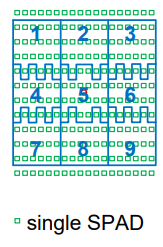
\includegraphics[height=4cm]{media/03_technical_implementation/SPAD-Map_6.png}
            \end{center}
            \caption{Schema der verwendeten SPAD Map\protect\footnote{Quelle: https://cdn.sparkfun.com/assets/learn\_tutorials/2/2/8/9/TMF882X\_DataSheet.pdf}}
            \label{fig:SPAD-Map_6}
        \end{figure}

        Da bei dieser SPAD Map Konfiguration der vertikale Messwinkel größer ist als der horizontale Messwinkel muss der Sensor für einen maximal großen Messbereich um 90° versetzt eingebaut werden, sodass die Messfelder 1, 4 und 7 die obere Messreihe bilden und die Messfelder 3, 6 und 9 die untere. Da jedoch auch der horizontale Messwinkel mit 41° einen großen Messbereich abdeckt, der nach der Rotation in der Vertikalen aufgespannt ist, wird die daraufhin obere Messebene mit den Feldern 1, 4 und 7 bei der Messung nicht ausgewertet, da dieser Messbereich zu großen Teilen oberhalb der Einwurföffnung gelegen ist. Die zwei geforderten Messebenen sind somit durch die Messbereiche 2, 5 und 8 für die obere Messebene sowie 3, 6 und 9 für die untere gegeben.\\

        Die Implementation der abstrahierten Interaktion mit dem Sensor ist in der Datei tmf8821.cpp realisiert, die entsprechende Schnittstelle dazu durch die Header Datei tmf8821.hpp gegeben. Durch die dort definierte Methode init wird der Sensor konfiguriert. Das bedeutet, die SPAD Map wird auf die vordefinierte SPAD Map mit der ID 6 festgelegt und der zeitliche Abstand zwischen zwei Messungen wird auf 50\,ms gesetzt. Dieser Wert hat sich aus Testläufen mit unterschiedlichen Werten ergeben. Das Ziel ist diesen Wert so gering zu halten wie möglich, damit ein eingeworfener Gegenstand auf jeden Fall detektiert wird und nicht genau zwischen zwei Messungen eingeworfen werden kann. Die durchgeführten Tests haben ergeben, dass Messungen mit einem zeitlichen Abstand von unter 50\,ms jedoch ungenauere Messwerte hervorbrachten. Die init Methode sollte typischerweise in der Setup Methode der main Klasse aufgerufen werden.\\

        Die Methode start lässt den Sensor eine einzelne Messung durchführen und interpretiert zugleich das Ergebnis. Dazu werden die vom Sensor zurückgelieferten Messwert zu einem Status ausgewertet, welcher in der aktuellen Instanz des Sensorobjekts gespeichert wird. Dabei kann das Messergebnis einem von drei möglichen Status zugeordnet werden. Die Status und ihre Bedeutungen werden in folgender Tabelle erläutert.\\

        \begin{table}[H]
            \centering
            \begin{tabularx}{\textwidth}{ |l|X| } 
                \hline
                NONE & In keiner der beiden auszuwertenden Messreihen wird ein Objekt detektiert.\\
                \hline
                INCOMING & In der oberen Messebene wurde ein Objekt detektiert. \\
                \hline
                DETECTED & Der vorherige Zustand ist INCOMING und in der unteren Messebene wird ein Objekt detektiert, während in der oberen Messebene keines mehr detektiert wird. Dieser Zustand kann nicht mehr durch weitere Messungen geändert werden, sondern wird beim Auslesen des Sensorzustandes zurückgesetzt.\\
                \hline
            \end{tabularx}
        \end{table}

        Um den Zustand des Sensors auszulesen, kann die Methode getState aufgerufen werden. Diese gibt immer den aktuell gespeicherten Zustand zurück. Ein Parameter vom Typ bool gibt an, ob der Zustand auf NONE zurückgesetzt werden soll, wenn der aktuelle Zustand DETECTED ist. Diese Option dient lediglich Debug Zwecken und im Produktivsystem sollte die Methode grundsätzlich nur mit dem bool-Wert true aufgerufen werden, da ein Aufruf der getState Methode mit einem Parameterwert von true die einzige Möglichkeit ist, den DETECTED Zustand zurückzusetzen.\\
        
        Während des Verlaufs der technischen Umsetzung wurde deutlich, dass die Bedienung des Einwurfsensors durch den Arduino nur dann in entsprechend schneller Taktung erfolgen kann, wenn der Arduino keine weiteren Aufgaben erfüllen muss. Somit musste für die Steuerung und Auswertung des Einwurfsensors ein eigenständiger Arduino, im folgenden Sensor-Arduino genannt, eingesetzt werden, welcher über zwei digitale Leitungen mit einem zweiten Arduino, im folgenden Haupt-Arduino genannt, kommuniziert, der die restlichen Funktionen des Gerippten steuert. Eine der Leitungen wird vom Sensor-Arduino auf HIGH gesetzt, sobald der Status DETECTED ausgelesen wird. Wenn der Haupt-Arduino diesen Status erkannt hat, setzt dieser die zweite Leitung für eine Iteration seiner main loop auf HIGH, um die Meldung zu bestätigen. Diese Bestätigung wird wiederum vom Sensor-Arduino gelesen, woraufhin dieser die erste Leitung wieder auf LOW setzt. Somit dient der Sensor-Arduino dem Einwurfsensor als Steuergerät, welches dem Haupt-Arduino lediglich mitteilt, wann ein Einwurf detektiert wurde.\\

        Während der letzten Praxistests, im Endzustand der Modellbauphase wurde deutlich, dass die Messgeschwindigkeit für die Einwurfdetektion noch nicht ausreichend ist, um Einwürfe zuverlässig zu detektieren. Ein großer Teil der Einwürfe wurde nicht erkannt. Jedoch wurden 'falsche Einwürfe', bei denen beispielsweise die Hand hineingesteckt und wieder herausgezogen wurde, zuverlässig als nicht vollständige Einwürfe erkannt. Da es für die Vorstellung des Prototypen von Vorteil war eine zuverlässige Einwurfdetektion zu präsentieren, statt des zuverlässigen Ausschließens von nicht vollständigen Einwürfen wurde, die Bedingung für das Setzen des Detektionssignals angepasst, sodass jedes Mal ein Detektionssignal gesetzt wird, sobald der Sensorstatus nicht mehr NONE entspricht, was der Funktionsweise einer einzelnen Lichtschranke entspricht. Durch weitere Analyse des Quellcodes im Anschluss an die Präsentationsveranstaltung fiel auf, dass in der Methode start, zu sehen in Listing \ref{lst:tmf8821_start}, alle Messwerte mindestens doppelt und maximal vierfach durchlaufen werden, wenn der Sensorstatus vor der Messung den Wert INCOMING aufweist, da jeder Aufruf von checkMiddleRow oder checkBottomRow jeweils einmal über alle Messwerte der letzten Messung iteriert.\\
        
        \begin{listing}
            \begin{minted}{cpp}
            
void TMF8821::start(void)
{
    sensor.startMeasuring(results);
    IntakeState curr = state;
    switch (curr) 
    {
        case NONE:
            if (checkMiddleRow())
            {
                state = INCOMING;
            }
            break;
        case INCOMING:
            if (checkBottomRow() && !checkMiddleRow())
            {
                state = DETECTED;
            }
            else if (!checkBottomRow() && !checkMiddleRow())
            {
                state = NONE;
            }
            break;
        default:
            break;
    }
}
            
            \end{minted}            
            \caption{start Methode aus tmf8821.cpp ohne Kommentare und Logging Ausgaben}            
            \label{lst:tmf8821_start}            
        \end{listing}

        Die Auswertung der Messwerte zum neuen Status kann jedoch auch mit einer einzelnen Iteration über die Messdaten realisiert werden, indem die Methoden checkMiddleRow und checkBottomRow zu einer Methode zusammengefasst werden, die einmal durch die Messwerte iteriert und dabei zurückgibt in welchen Messebenen etwas detektiert oder eben nichts detektiert wurde. Diese Verbesserung bietet somit eine Reduktion der Laufzeit, welche möglicherweise ausreichend ist, um die Einwurfdetektion in ihrem geplanten Zustand funktionsfähig zu implementieren.
        
\section{Detektion von Flaschen im Flaschenring}
    \subsection{Diskussion}
        Bei der Detektion von Flaschen im Flaschenring ist zu beachten, dass hierfür ein Sensor verwendet werden muss, der Glas in verschiedenen Farben einwandfrei detektiert. Es zeigt sich, dass sowohl die meisten optischen Sensoren, als auch Ultraschallsensoren dazu in der Lage sind. Bei optischen Sensoren ist jedoch zu bedenken, dass die maximale Detektionsreichweite bei der Detektion von Glas kleiner sein kann, als vom Hersteller angegeben, da die Reflektivität von Glas, je nach dessen Einfärbung, nicht sehr hoch ist. Somit ist ein Ultraschallsensor für die Detektion von Flaschen die zuverlässigere Wahl.\\

        Ein weiteres Kriterium, welches vom Sensor erfüllt werden sollte, ist eine geringe Komponentengröße, da er sonst nicht ohne großen Aufwand zwischen Flaschenring und Tonnenkörper montiert werden kann. Das Sensormaß entlang seiner Messachse ist hierbei besonders ausschlaggebend.\\

        Die kleinsten Ultraschallsensoren die während der Komponentenrecherche ermittelt wurden besitzen Bauhöhen von einem bis zu zwei Zentimetern, während der flachste Lidarsensor der ermittelt wurde ein Bauhöhe von 3\,mm besitzt. Dabei handelt es sich um Digital Distance Sensor von Pololu. Welcher, aufgrund ebendieser geringen Bauhöhe und trotz der Einschränkung, dass die Reichweite eventuell geringer ausfällt, als vom Hersteller angegeben, für dieses Projekt ausgewählt wurde. Dieser Sensor wird in verschiedenen Ausführungen angeboten, wobei diese sich in ihrer maximalen und minimalen Messdistanz unterscheiden. Da es sich um einen Sensor mit digitalem Ausgangssignal handelt und somit nur detektiert wird, ob ein Objekt vorhanden ist und nicht wie weit es entfernt ist, muss sichergestellt sein, dass die Reichweite gering genug ist um nicht die, dem Sensor gegenüberliegende, Wandung des Flaschenfachs zu detektieren, da der Sensor seitlich am Flaschenfach angebracht wird. Da die Flaschenfächer zum Zeitpunkt der Materialauswahl nicht vollständig konzipiert waren, wurde die Sensorvariante ,mit einer Reichweite zwischen 0,5\,cm und 5\,cm ausgewählt und damit der Durchmesser der Flaschenfächer auf mindestens 5\,cm festgelegt. Die Polou Teilenummer dieser Sensorvariante ist 4050.\\
        
        Wie bereits erwähnt, wird der Sensor seitlich an den Fächern des Flaschenrings montiert. Eine Montage an der Unterseite des Fachs wurde ausgeschlossen, da dies sehr fehleranfällig ist. Beispielsweise könnte sich Dreck am Boden des Fachs sammeln und den Sensor somit blockieren. Da der Sensor zwischen Flaschenring und Tonnenkörper montiert wird und der Flaschenring eine leichte Neigung nach außen aufweist, ist der Sensor von der Horizontalen Ebene nach unten abweichend ausgerichtet und somit gegen grobe Verschmutzungen, die von oben in das Fach gelangen geschützt.\\

    \subsection{Implementation}
        Die Datei pololu\_digi5.cpp implementiert die Headerdatei pololu\_digi5.hpp und ermöglicht die Abstratktion der Sensorfunktion in der Software. Eine Instanz dieses Sensors wird duch den Konstruktor initialisiert, welchem der entsprechende Arduino Anschlusspin übergeben wird. Da der Sensor ein hohes Potential an seinen Ausgangspin anlegt, solange nichts detektiert wird, wird der pinmode INPUT\_PULLUP verwendet, sodass das Signal am Eingangspin des Arduino ebenfalls hohes Potential besitzt, solange die angeschlossene Leitung das Signal nicht aktiv auf das niedrige Potenzial bringt.\\

        Die Methode read liest das Signal am entsprechenden Pin aus, negiert dieses und gibt das Ergebnis der Negation als bool Wert zurück. Die Negation wird durchgeführt, sodass ein Rückgabewert von true einer Detektion entspricht und ein Rückgabewert von false bedeutet, dass sich kein Objekt im Messbereich des Sensors befindet.

\section{Kommunikation zwischen Endgeräten} \label{communications}

    \subsection{Diskussion}
        Um die Kommunikation unter mehreren 

    \subsection{Implementation}

\section{Füllstandsmessung}
    \subsection{Diskussion}
        Zum Messen des Füllstandes soll ein Sensor, oder eventuell auch mehrere, an der Unterseite des Tonnendeckels befestigt werden. Bei der Füllstandsmessung ist zu beachten, dass er Füllstand an unterschiedlichen Positionen in der Tonne eine unterschiedliche Höhe aufweisen kann. Somit existiert kein einzelner korrekter Füllstandswert, wie es bei einer Flüssigkeit der Fall wäre. Daraus ergeben sich verschiedene Möglichkeiten für die Ermittlung eines Füllstandswertes. Eine dieser Möglichkeiten wäre, mehrere Messungen an unterschiedlichen Punkten durchzuführen und daraus einen Mittelwert zu bilden oder den Punkt mit dem höchsten Füllstand als aktuellen Wert anzunehmen. Eine weitere Möglichkeit besteht darin lediglich eine Messung an einer fixen Position durchzuführen. Diese Methode besitzt zwar eine gewisse Fehleranfälligkeit, da der Füllstand an einem anderen Punkt höher sein könnte, liegt der Messpunkt jedoch mittig, sollte in den meisten Fällen dort auch der aktuell höchste Füllstand ermittelt werden, da sich die Oberfläche des Mülls in der Tonne häufig zu einem sehr flachen Kegel auftürmt. Der klare Vorteil der Umsetzung mit einem Sensor liegt jedoch in der Einfachheit der Umsetzung dieser Methode, da nur ein Sensor benötigt wird und nicht mehrere Sensordaten miteinander verrechnet werden müssen.\\
        
        Es besteht zusätzlich die Möglichkeit auch für Füllstandsmessung den, im Abschnitt Einwurferkennung beschriebenen, Sensor TMF8821 von SparkFun zu verwenden, da dieser jedoch vergleichsweise hohe Kosten aufweist und eine Komplexität bietet, die von der Füllstandsmessung nicht zwingend gefordert wird, soll ein simplerer Sensor eingesetzt werden. Hierfür kommen sowohl optische als auch Ultraschallsensoren in Frage, die eine Reichweite von mindestens 140\,cm besitzen, da dies in etwa der Gesamthöhe des Gerippten entspricht. Die Auswahl der Sensoren bei den von uns ausgewählten Zulieferern war im unteren Preissegment nicht besonders groß, weshalb wir uns für den Sharp GP2Y0A60SZLF Analog Distance Sensor auf einem Pololu Carrier entschieden. Dabei handelt es sich um einen optischen Sensor mit einer Reichweite von 10\,cm bis 150\,cm. Das Ausgangssignal des Sensors ist analog.\\

        Die Füllstandsmessung ist eine Funktion des Gerippten, die in diesem Projekt jedoch keine weitere Außenwirkung aufweisen soll, und wird lediglich implementiert um das Konzept eines smarten Mülleimers zu verdeutlichen. In einer weiteren Umsetzung können die Daten zum Füllstand dann beispielsweise an eine zentrale Steuereinheit übertragen werden. Weitere Informationen zur möglichen Weiterführung des Projekts befinden sich im Kapitel Zukünftige Entwicklungsmöglichkeiten.\\

    \subsection{Implementation} 
        Die Interaktion mit dem Sensor wird im Quellcode in der Datei level\_meter.cpp implementiert. Diese implementiert wiederum die Headerdatei level\_meter.hpp. Um eine Instanz des Sensors zu initialisieren muss dem Konstruktor zum einen der Anschlusspin des Arduinos übergeben werden und weiterhin die Abstandsmaße vom Sensor bis zum leeren Füllstand, sowie bis zum vollen Füllstand. Dabei ist zu beachten, dass der Abstandswert zwischen Sensor und vollem Füllstand mindestens 10\,cm betragen sollte, da dies die minimale Messdistanz des Sensors ist.

        Desweiteren existiert die Methode calculateDistance, welche den vom Sensor ausgegebenen Wert am Arduino Pin einliest und daraus die Distanz zum detektierten Objekt errechnet. Für die Implementation dieser Methode musste jedoch zuerst ermittelt werden, wie ein Signalwert in einen Distanzwert umgerechnet wird. Dazu wurde der Sensor auf einem Breadboard befestigt und mit dem Arduino verbunden. Der Sensor wurde auf einer ebenen Fläche so ausgerichtet, dass seine Messebene parallel zum Untergrund verläuft. Danach wurde vor dem Sensor eine weißer Karton im Abstand von 10\,cm platziert. Der Arduino wurde so konfiguriert, dass der Sensorwert alle 25\,ms 500 mal nacheinander ausgelesen wird. Dabei wird der Mittelwert der 500 Messungen berechnet und vom Arduino auf dem seriellen Monitor ausgegeben. Dieses Vorgehen wurde mit, in 5\,cm Schritten, steigenden Abständen zum Karton wiederholt, bis zu einem maximalen Abstand von 150\, cm. Die gemessenen Durchschnittswerte wurden im Programm Excel von Microsoft eingepflegt. Dort wurde aus den Daten ein Diagramm, inklusive Trendlinie und Trendlinienformel erstellt. Die Ergebnisse sind in Tabelle \ref{tab:calibration} und Abbildung \ref{fig:calibration} zu sehen.

        \begin{table}
            \centering
            \caption{Ergebnisse der Abstandsmessungen}
            \begin{tabular}{ c c } 
                Distanz (cm) & Messwert\\ [0.5ex]
                \hline
                \hline
                10 & 574\\
                15 & 423\\
                20 & 343\\
                25 & 310\\
                30 & 303\\
                35 & 300\\
                40 & 294\\
                45 & 287\\
                50 & 279\\
                55 & 273\\
                60 & 265\\
                65 & 259\\
                70 & 253\\
                75 & 249\\
                80 & 243\\
                85 & 238\\
                90 & 235\\
                95 & 231\\
                100 & 226\\
                105 & 223\\
                110 & 219\\
                115 & 216\\
                120 & 214\\
                125 & 211\\
                130 & 209\\
                135 & 207\\
                140 & 204\\
                145 & 203\\
                150 & 202\\
            \end{tabular}            
            \label{tab:calibration}
        \end{table}

        \begin{figure}[H]
            \begin{center}
                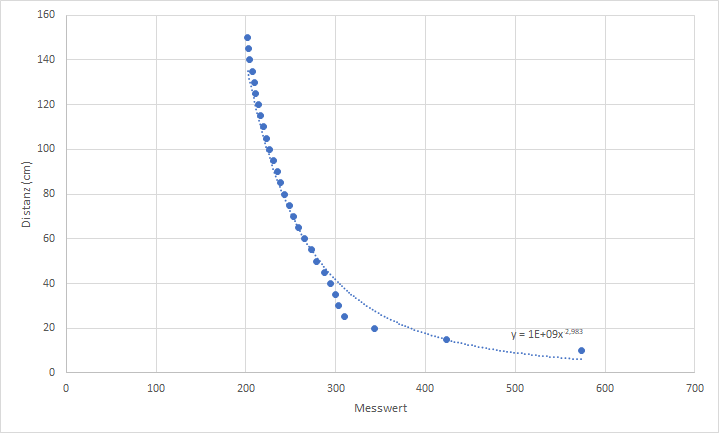
\includegraphics[width=12cm]{media/03_technical_implementation/calibration.png}                
            \end{center}
            \caption{Von Microsoft Excel generierter Graph auf Basis der Messdaten}
            \label{fig:calibration}
        \end{figure}

        Es zeigt sich, dass die Trendlinie, insbesondere bei den kurzen Distanzen, den Messpunkten sehr gut folgt. Bei den mittleren Distanzen gibt es leichte Abweichungen, da dort auch die Messpunkte keinem klar erkennbaren Muster folgen. Das führt dazu, dass die Messungen, insbesondere in diesem Bereich, kein sehr genaues Ergebnis liefern werden. Jedoch werden die Abweichungen vom Ist-Zustand auch nicht so groß sein, dass die Messwerte für eine Auswertung, durch beispielsweise die FES, unbrauchbar sind. Der größte Nutzen der Füllstandsmessung, das Detektieren einer vollen Tonne, ist einwandfrei gegeben, durch die Genauigkeit der Trendlinie bei kurzen Distanzen.\\

        Die für den Füllstandssensor implementierte Methode getFillLevel ruft die bereits angesprochene Methode liest den Messwert des Sensors aus und lässt anhand der bereits angesprochenen Methode calculateDistance die gemessene Distanz berechnen. Aus der gemessenen Distanz, der Distanz für den vollen Zustand und der Distanz für den leeren Zustand wird dann der Füllgrad berechnet und als abgerundeter, ganzzahliger Teil von 100 zurückgegeben.

\addtocontents{toc}{\protect\setcounter{tocdepth}{2}}

\section{Stückliste}
    \begin{table}[H]
        \centering
        \begin{tabularx}{\textwidth}{ | l | X | }\hline
            \textbf{Menge} & \textbf{Bezeichnung} \\\hline
            4              & Arduino Nano 33 BLE \\\hline
            1              & Sparkfun Qwiic dToF Imager - TMF8821 \\\hline
            3              & Pololu 5cm Digital Distance Sensor \\\hline
            1              & Sharp GP2Y0A60SZLF Analog Distance Sensor 10-150cm \\\hline
            30             & Adafruit Neopixel RGBW 0.2W \\\hline            1              & Adafruit NeoPixel RGB LED Strip 30 LEDs/m 5m \\\hline
            2              & Level Shifter, Joy-IT TXB0104 \\\hline
            1              & Netzteil POS-50-5-C 5V 10A \\\hline
            5              & Solderable Breadboards \\\hline
            40 Meter       & 0.75mm\textsuperscript{2} Kupferkabel - verschiedene Farben \\\hline
            1 Meter        & 1.5mm\textsuperscript{2} Kupferkabel - verschiedene Farben \\\hline
            ca. 170        & Crimps \\\hline
            ca. 50         & Stecker \\\hline
        \end{tabularx}
    \end{table}

\section{Schaltpläne}
    In den folgenden Grafiken wird die Verschaltung der Arduino Mikrocontroller mit den Sensoren und Leuchtmitteln dargestellt. Dabei ist in Abbildung \ref{fig:circuit_diagram_transmitter} die Verschaltung der Komponenten der großen Gesamtmodells zu sehen, während Abbildung \ref{fig:circuit_diagram_receiver} den Schaltplan des kleinen Rautenmodells zur Präsentation der Bluetoothkommunikation zeigt.

    \begin{figure}[H]
        \begin{center}
            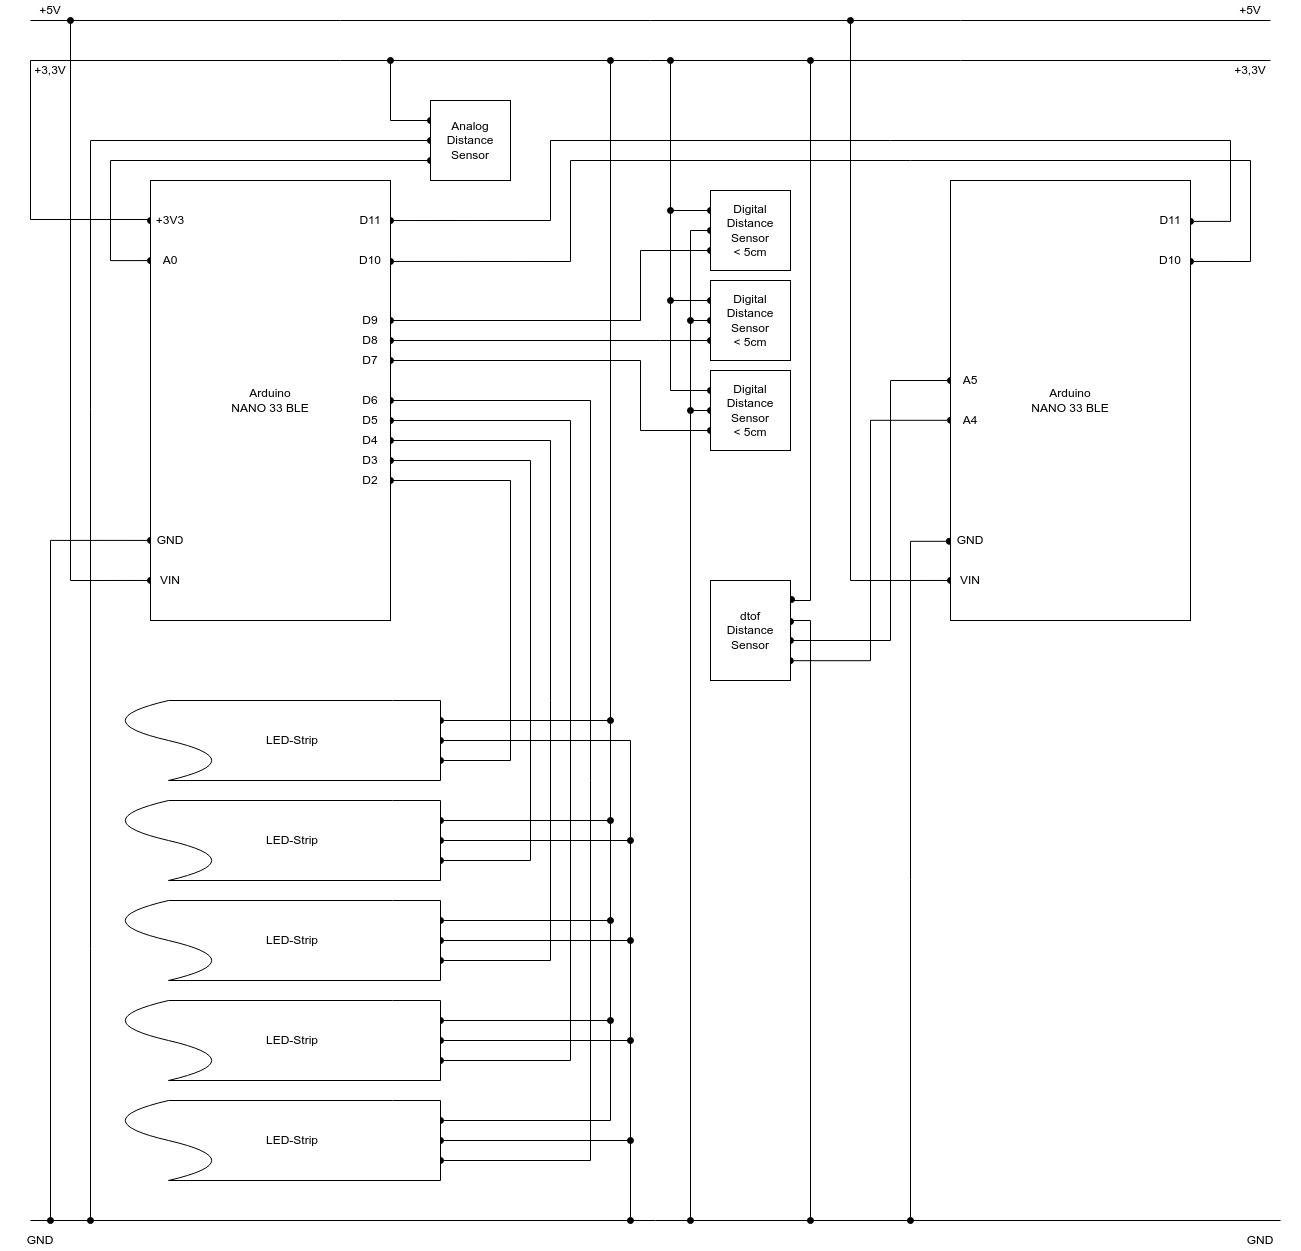
\includegraphics[width=\textwidth]{media/03_technical_implementation/circuit_diagram_transmitter.png}
        \end{center}
        \caption{Schaltplan des Hauptmodells}
        \label{fig:circuit_diagram_transmitter}
    \end{figure}

    \begin{figure}[H]
        \begin{center}
            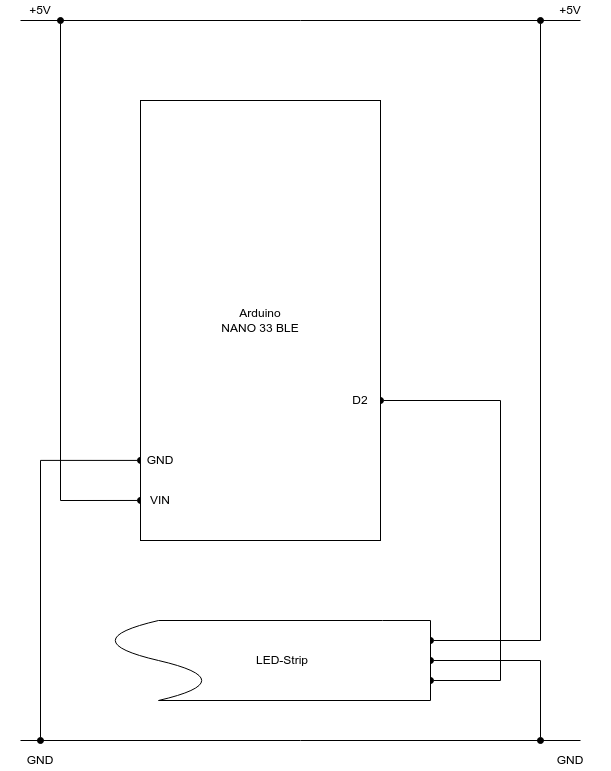
\includegraphics[width=6.8cm]{media/03_technical_implementation/circuit_diagram_receiver.png}
        \end{center}
        \caption{Schaltplan der zwei Rauten Modelle}
        \label{fig:circuit_diagram_receiver}
    \end{figure}

\section{Zusammenführung von Modell und Technik}

    \subsubsection{Der Maschinenraum}
        
        Für die zwei Arduinos, das Netzteil und die Breadboards für die Steckverbindungen unserer Sensoren und LEDs brauchen wir im Mülleimer einen geschützten Ort. Wir haben uns dafür entschieden, diesen \enquote{Maschinenraum} im Boden der Tonne zu platzieren, und einen um 10 Zentimeter erhöhten Doppelte-Boden einzubauen, auf dem dann die innere Mülltonne steht.
        So kann man die innere und danach die äußere Tonne nach oben rausheben, da beide Böden nicht fest mit der Tonne veranker sind.
        Damit kommen wir immer an unsere Technik.
        Dann habe wir am unteren Rand der Tonne noch ein Loch für unsere Stromverkabelung geschnitten, sodass das das einzige Kabel ist, was von außen sieht.

    \subsubsection{Verkabelung}

        Die restlichen Kabel sind an der Innenwand der äußeren Tonne nach oben gezogen und dann dort durch kleine Löcher nach Bedarf nach außen geführt.


    \subsubsection{Technik im Flaschenring}

        Die LEDs der Fächer im Flaschenring haben wir von unten außen an die Konstruktion geklebt und vorher passende Löcher in die Fächer geschnitten. Analog dazu sind wir bei den 5cm Lidar Sensoren an der Rückseite der Fächer vorgegangen. (Zwischen Tonnenwand und Flaschenring.)

    \subsubsection{LED-Strips}

        Da die Rauten unterschiedliche Kantenlängen zwischen 8 und 10,5cm besitzen, die LED-Strips aber parallel zum Modellbau gelötet werden mussten, brauchten wir einen Ansatz der einen gewissen Spielraum ermöglicht. Ebenfalls unbekannt war, in wiefern die Rautenstruktur aus Schaumstoff anpassbar waren, da wir zu dem Zeitpunkt darüber noch keine Informationen bekommen hatten.
        Wir haben daher zwischen den geteilten LED-Strips längere Kabelverbindungen als nötig verwendet, denn während wir unter perfekten Umständen die Abstände der Übergange zwischen zwei Rauten hätten ausmessen können und wir die Kabel damit unter oder an den Rauten hätten verlegen können, müssen wir so die Länge der Kabel an jedem Übergang zweier Strips variieren können.
        Umgesetzt wurde das, in dem wir an jeder dieser Übergänge ein etwa 8mm dickes Loch in die Tonne gebohrt haben, um das übrige Kabel als Schlaufe in die Tonne zu führen. Die benötigte Drehung des LED-Strips um die Lötpunkte und Kabel in die Richtung des Lochs zu drehen, haben wir vorsichtig am LED-Strip selbst gebogen.
        Die langen Strecken, an denen das Kabel auf eine andere Höhe gebracht  werden mussten (zu sehen in Abbildung\,\ref{fig:led_wiring_rhombus}) hatten wir ursprünglich geplant außen an der Raute langzuführen und an beiden Enden der Kante jeweils eine Schlaufe in die Tonne führen zu lassen, sodass wir die LED-Strips einfacher hätten abmontieren können.
        Unter der Voraussetzung, dass wir die Strips an dem Schaumstoff der Rauten festgeklebt wurde, haben wir uns aus ästhetischen Gründen dazu entschieden die Kabel an den langen Kanten in der Tonne langzuführen.


\chapter{Ergebnis} \label{summary}

\section{Der Gerippte} 
    Durch eine intensive Schlussphase konnten wir unsere drei anfänglich beschrieben Funktionen fertigstellen. (Siehe \ref{cpt:funktionen})

    Wir haben drei unserer Flaschenringfächern mit Sensoren ausgestattet um die Funktionalität vorzuführen, während alle Fächer mit jeweils 2 LEDs ausgestattet wurden. So konnten wir ebenfalls die ästhetische \enquote{Flaschen-Krone} präsentieren. Die weiß beleuchteten Flaschen haben den von uns erwünschten Eindruck erfüllt und es war ein belohnendes Gefühl den Flaschenring mit Flaschen zu füllen.

    Ebenfalls fertiggestellt haben wir den Einwurfsensor, welchen wir kurz vor der Präsentation in der AMD im vollständig zusammengesetzten Zustand erfolgreich testen und dem anwesenden Prof vorführen konnten.
    Als Antwort auf einen Einwurf konnten wir eine Animation über die gesamte Raute abspielen. Dabei ist uns aufgefallen, dass der obere der drei Kabelstränge beim Einbau trotz Heißklebepunkten auf den Kontakten ein Wackelkontakt entwickelt hat, der die drei Farbwerte aus der Synchronität bringt. Da wir den Ursprung in der verleibenden Zeit nicht finden konnten, mussten wir uns entscheiden, nur eine der drei Farbkanäle anzusteuern. So haben wir uns für blaue Animationen entschieden.

    Ein weiteres Problem ist beim Abbau der Tonne für den Transport aufgetreten. Beim herausnehmen der inneren Tonne gab es erneut Probleme mit den LED-Strips. Diesmal gab es im unteren Kabelstrang Kontakt zwischen Strom und Erdung eine Verbindung, wodurch der LED-Strip extrem heiß wurde. Auch hier konnten wir leider keine Fehleranalyse mehr durchführen und mussten den unteren Teil für die anstehende Präsentation ausstecken.

    Auch erfolgreich umgesetzt haben wir die kleinen Rauten-Modelle, die andere Mülleimer simulieren sollten. Hier haben wir die Kommunikation zwischen dem Hauptmodell und einer Raute und parallel zwischen dem Hauptmodell und einem Handy, das die zweite Raute simuliert hat, mit dem in \ref{sec:communications} beschriebenem Ansatz getestet. Wir haben es aber nicht hinbekommen, beide Rauten anzuspielen. Den genauen Grund konnten wir uns, ebenfalls wegen der kurzen Zeit zur Abschlussveranstaltung, nicht mehr rekonstruieren.

    \begin{figure}[H]
        \begin{center}
            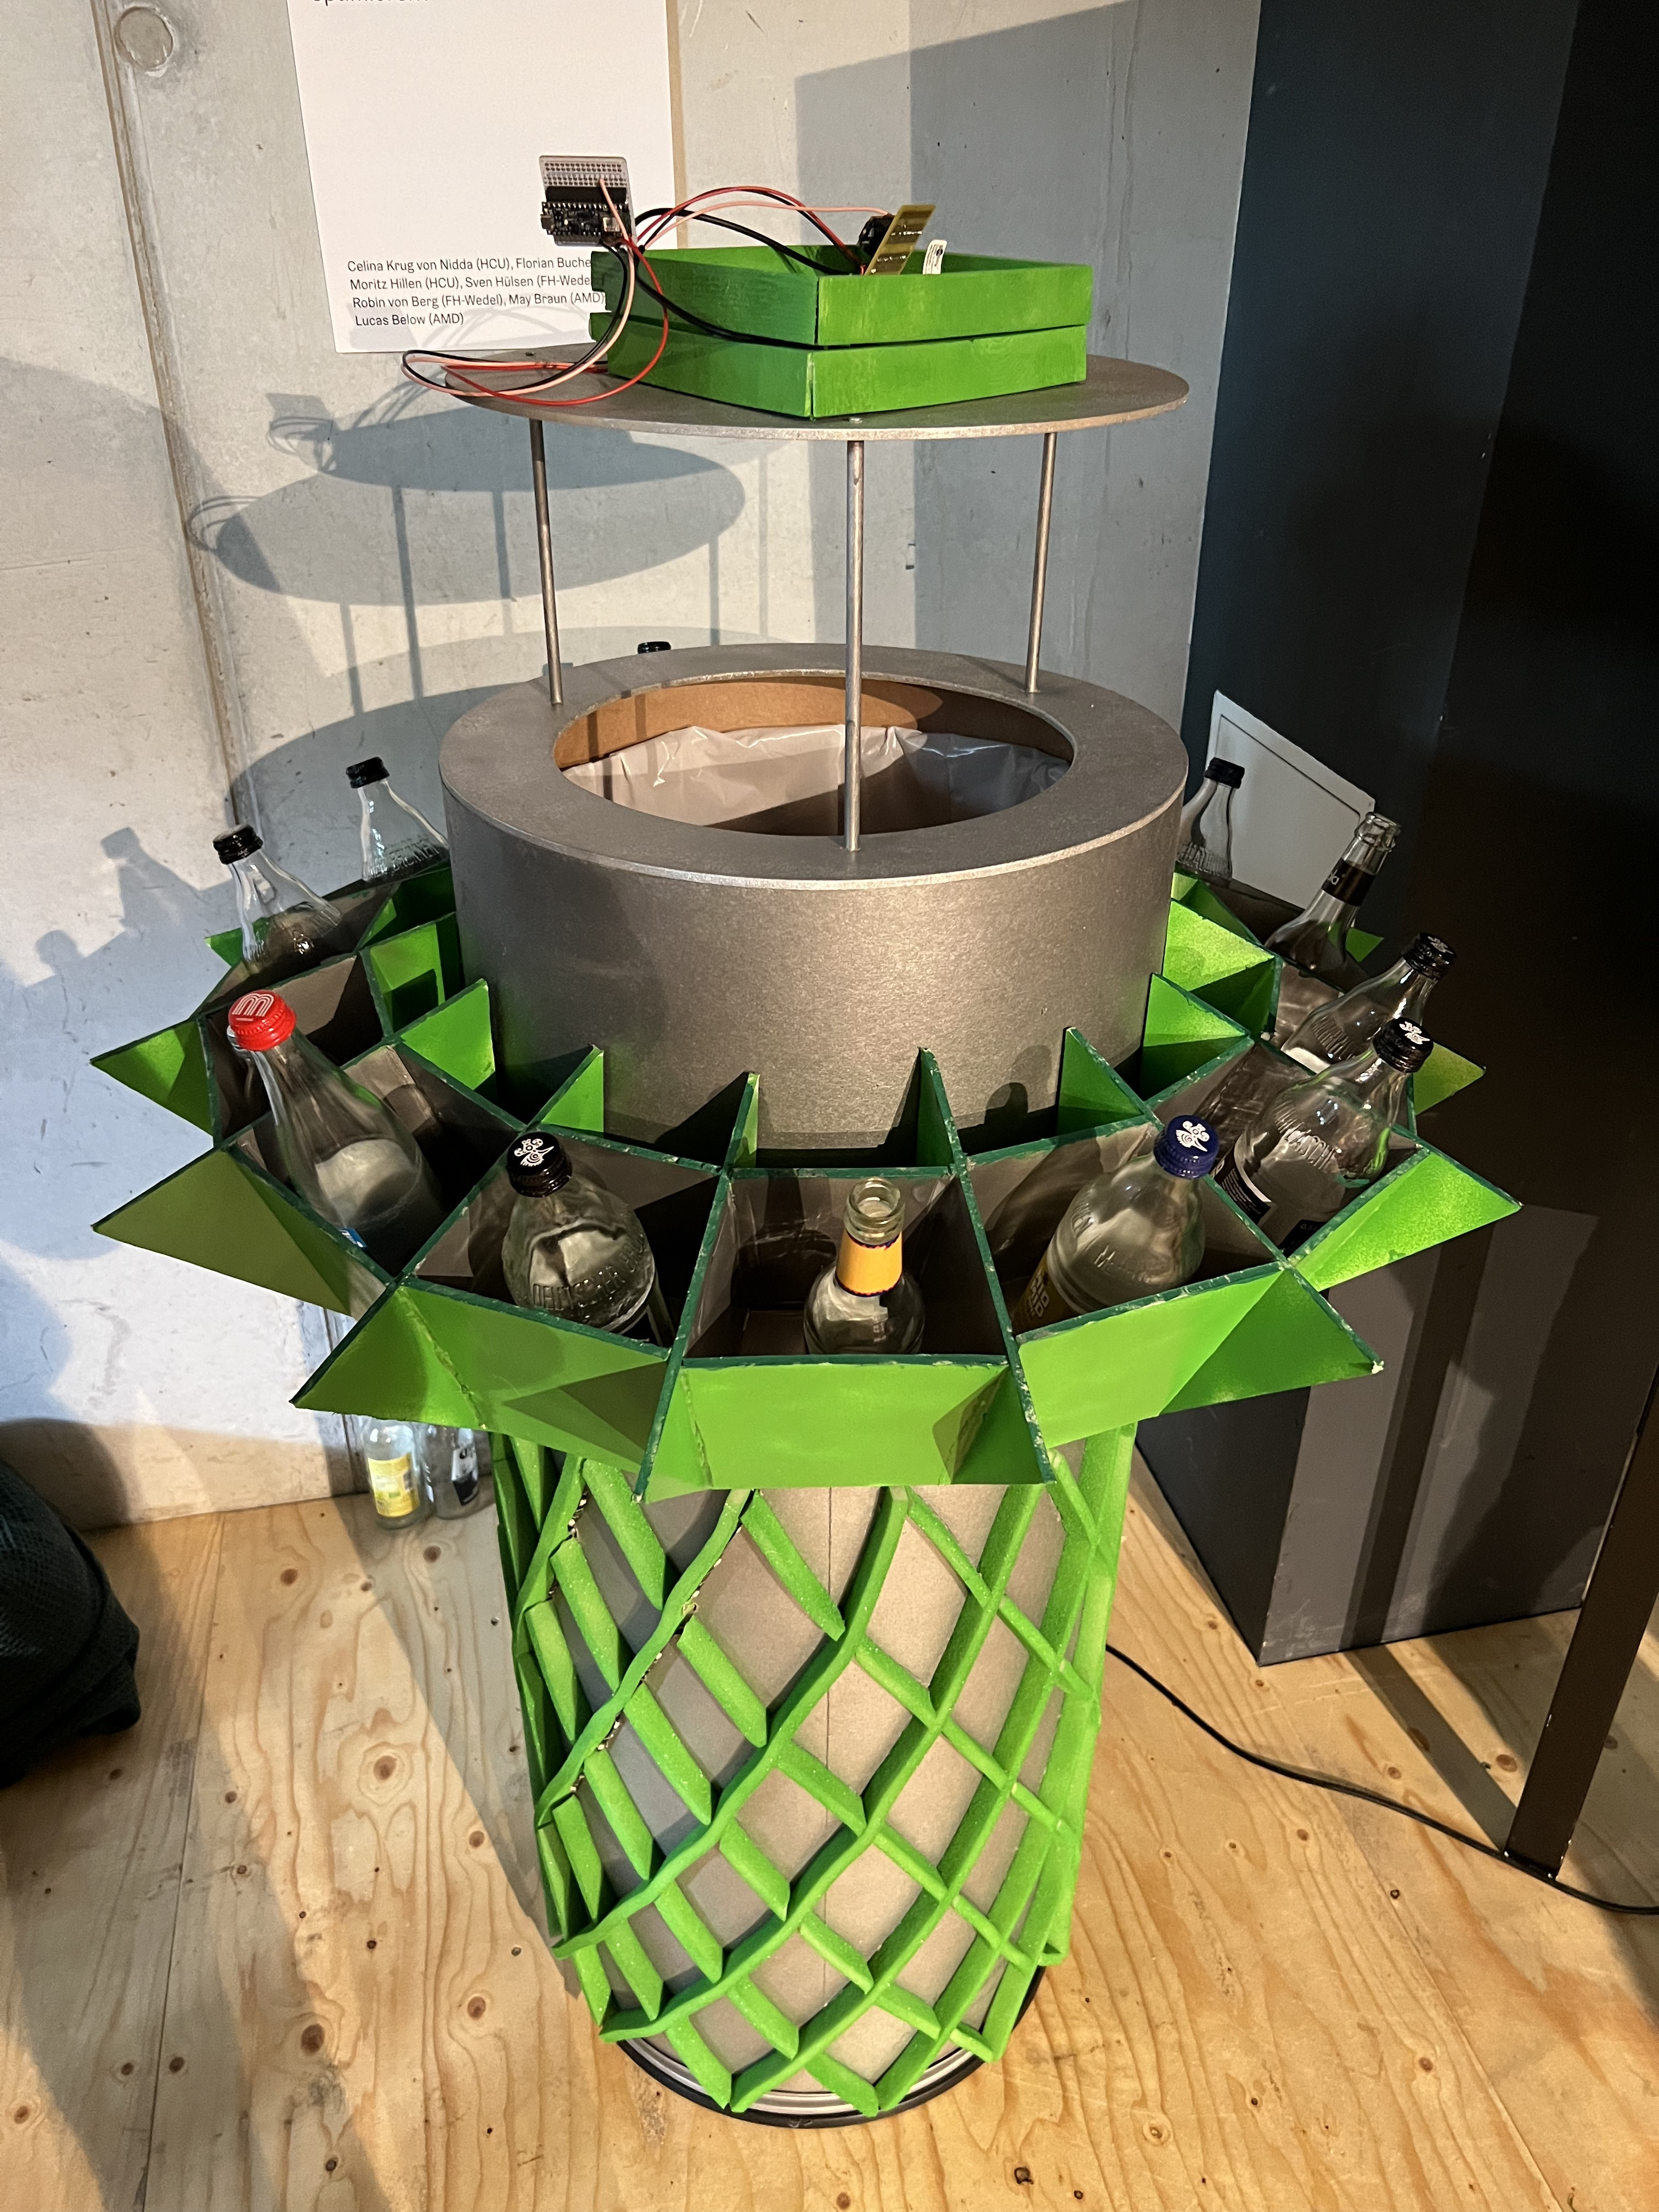
\includegraphics[width=6cm]{media/04_result/pic_bin.jpg}
        \end{center}
        \caption{Der Gerippte bei der Abschlussveranstaltung im betahaus mit den beiden Rauten auf dem Deckel.}
        \label{fig:pic_gerippte_1}
    \end{figure}

\section{Abschlussveranstaltung}

    \begin{figure}[H]
        \begin{subfigure}[b]{0.5\textwidth}
            \centering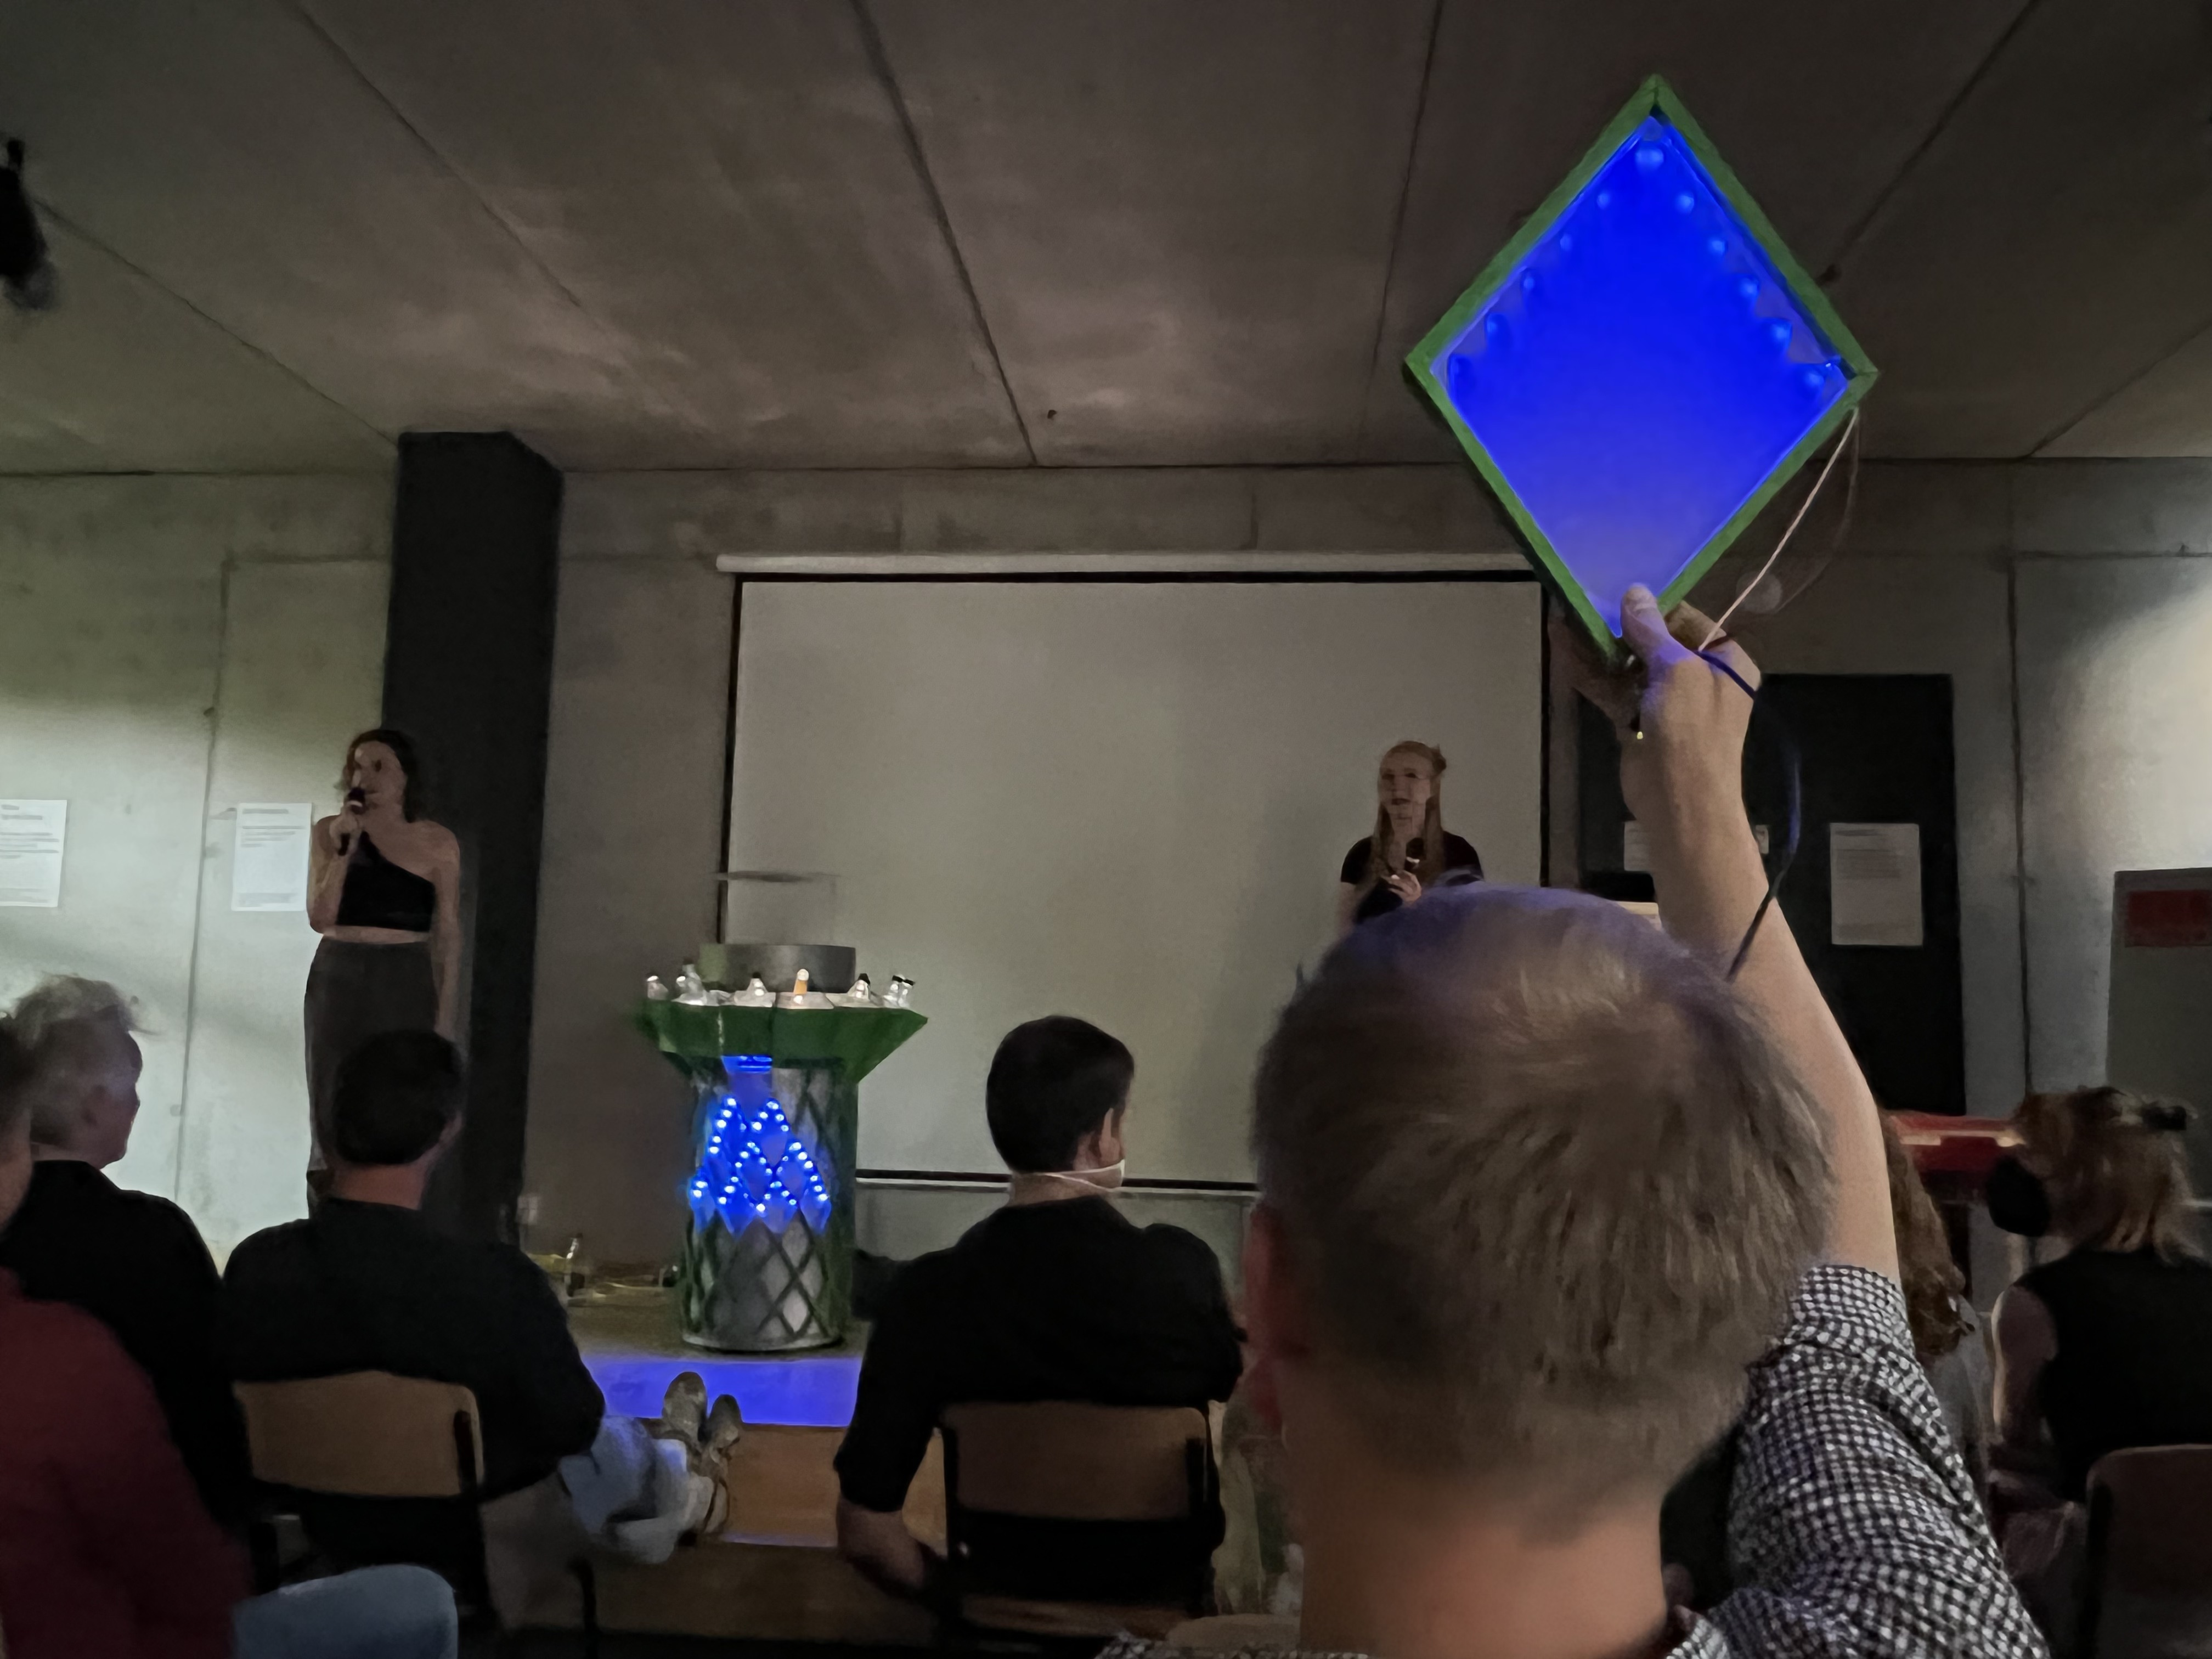
\includegraphics[width=\textwidth]{media/04_result/pic_communication.jpg}
            \caption{Unser Rauten-Modell in Aktion.}
            \label{fig:pic_gerippte_2}
        \end{subfigure}\quad
        \begin{subfigure}[b]{0.5\textwidth}
            \centering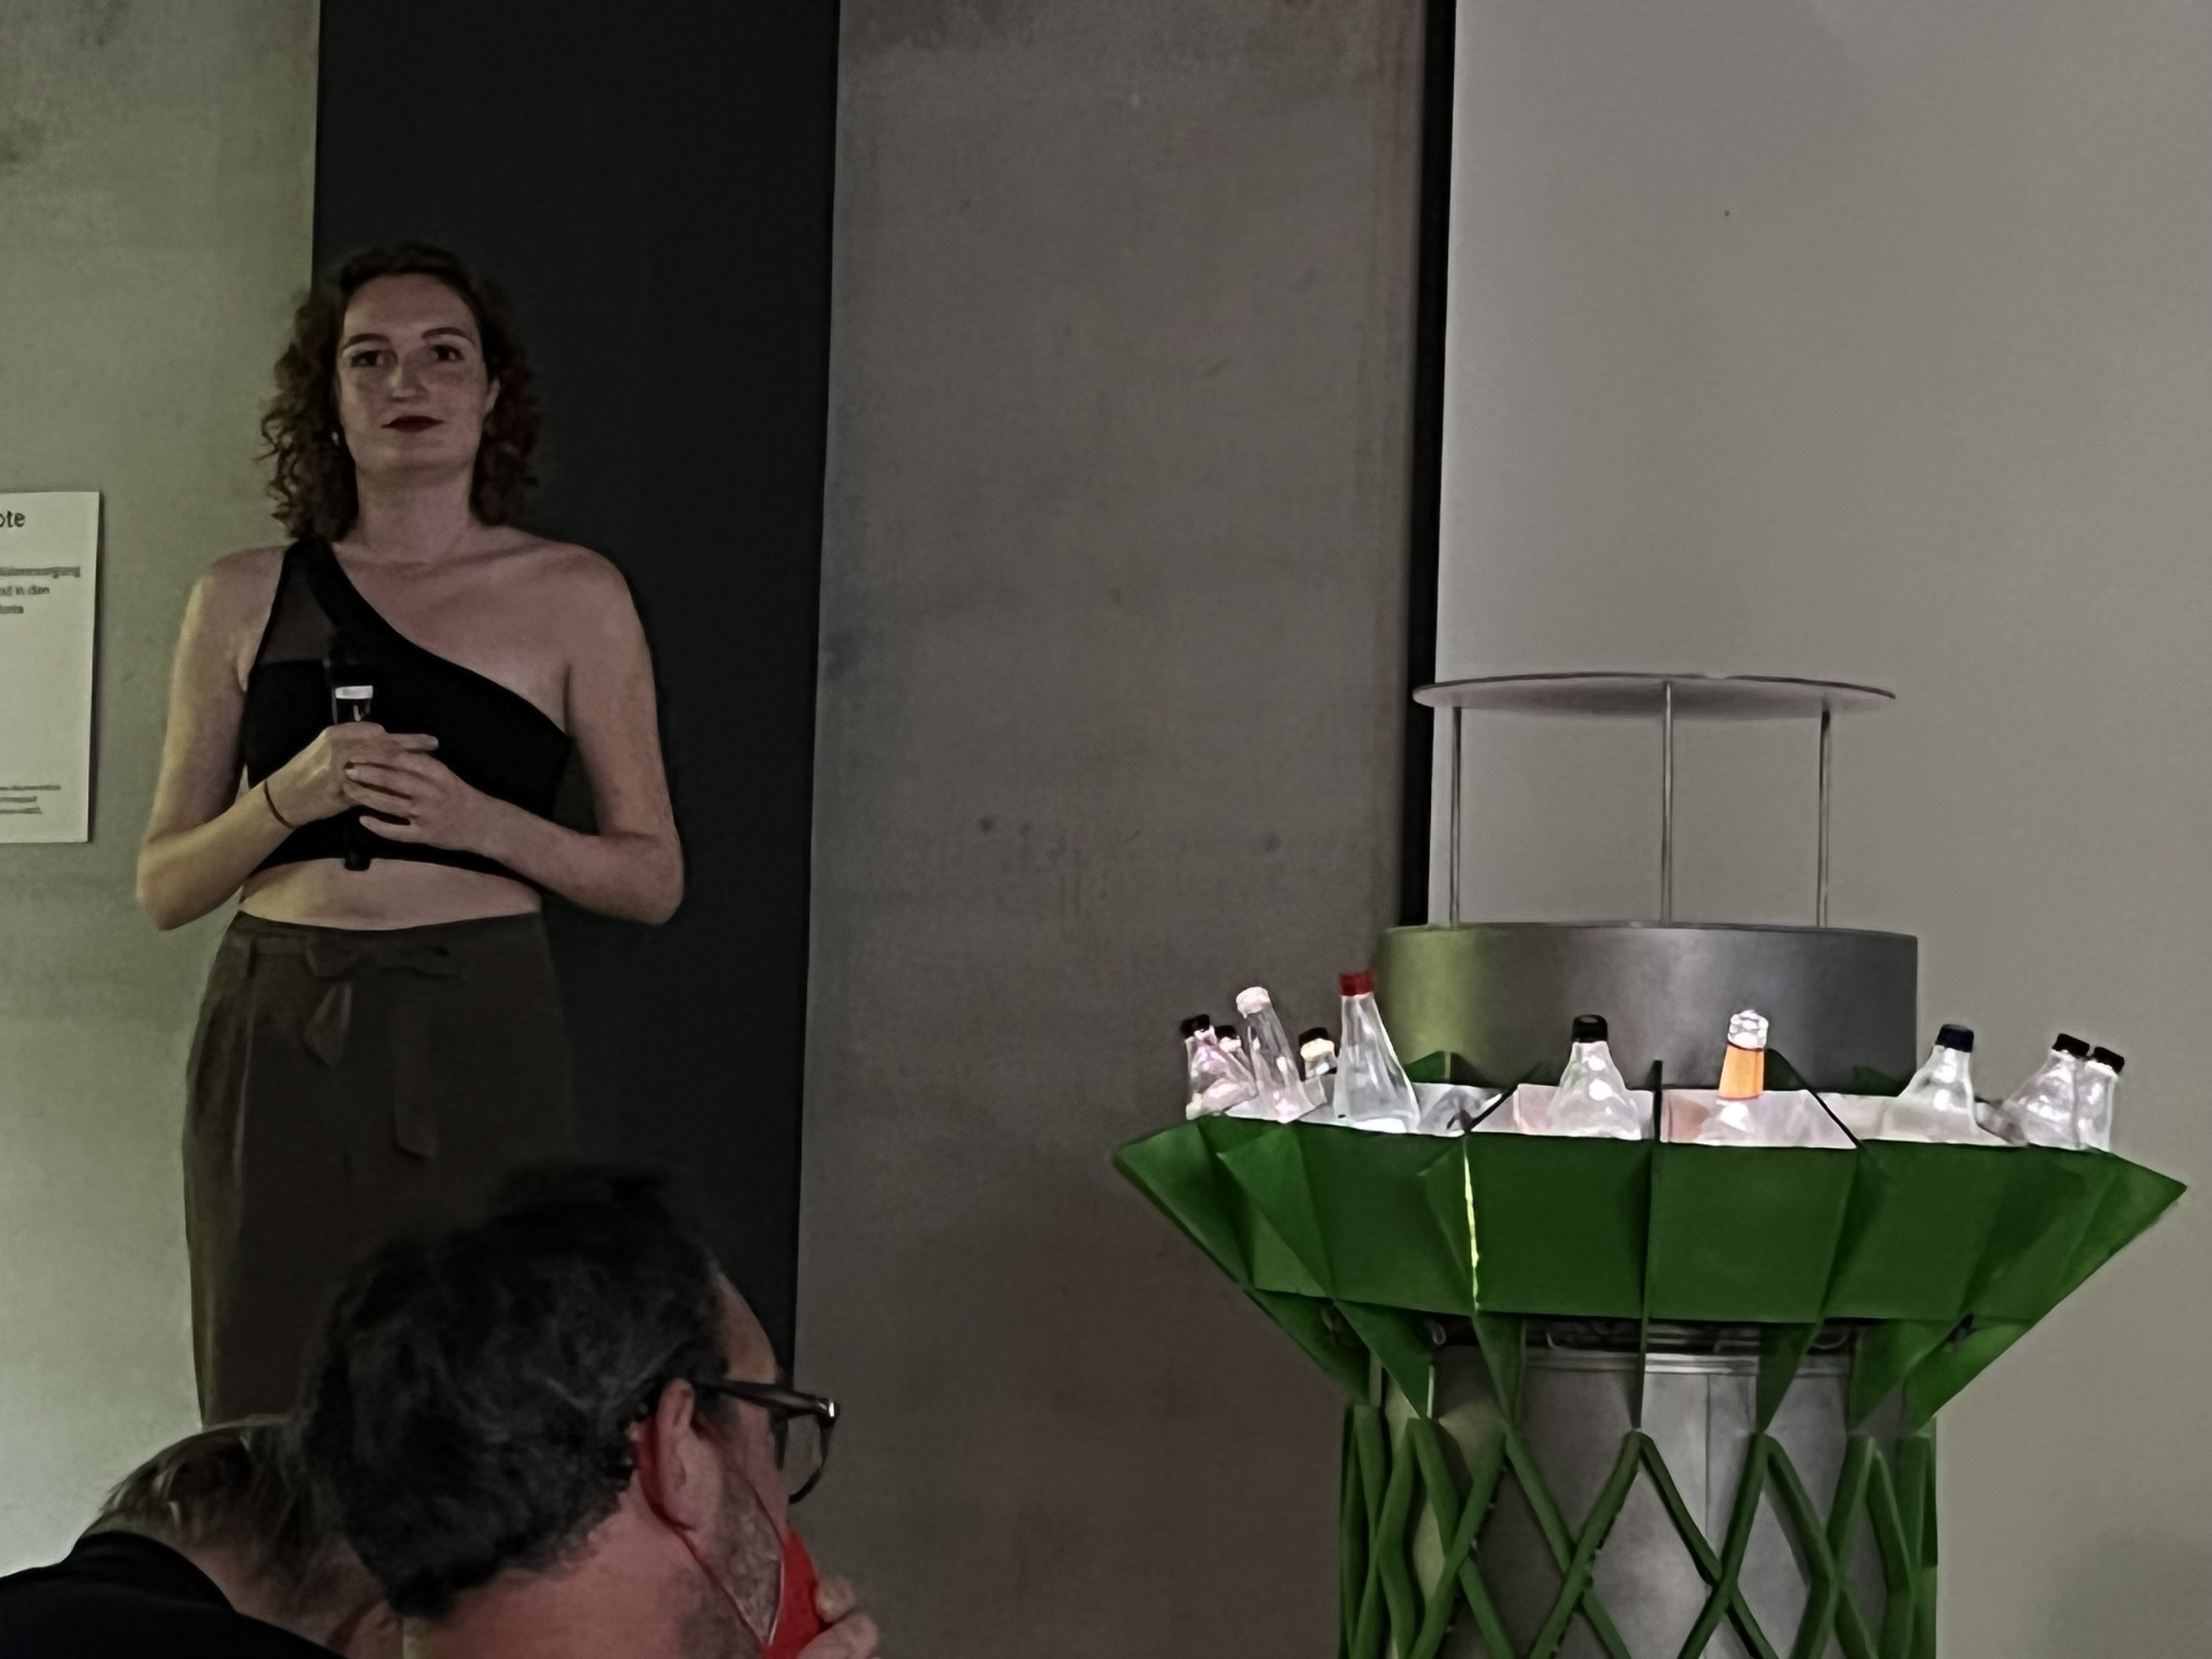
\includegraphics[width=0.7\textwidth]{media/04_result/pic_presentation_bottles.jpg}
            \caption{Beleuchtung der Flaschen im Flaschenring.}
            \label{fig:pic_gerippte_3}
        \end{subfigure}
        \caption{Eindrücke aus dem Pitch der Abschlussveranstaltung}
    \end{figure}

    Die im betahaus stattfindende Veranstaltung hat am \printdate{2022-06-30} um 18 Uhr stattgefunden. Hier haben alle 5 Teams ihre Modelle und Konzepte in einem sieben minütigem Pitch vorgestellt. Für unser Team haben Celina Krug und Maybritt Braun einen Pitch mit Unterstützung des Teams vorbereitet und dort hervorragend vorgetragen. Trotz eines unglücklichem Umstands, der Einwurfsensor hat, nachdem er vorher Vorort getestet wurde, während der Vorstellung dauerhaft ausgelöst, was unsere Funktionalität leider viel einfacher dargestellt hat, als sie im Hintergrund ablief.
    Der Grund der Fehlauslösungen liegt höchstwahrscheinlich in der Konfiguration des Sensors, denn auch wenn der maximale Abstand geringer eingestellt war, als die Kantenlänge des Sensorbereichs, kann es sein, dass diese Konfiguration im Sensor nicht fein genug umgesetzt werden kann und wir eine geringere Reichweite Wählen müssen.
        
\chapter{Fazit}

\section{Was lief gut}

\section{Was haben wir gelernt}
    Herausforderung bei der Realisierung
        Herausforderungen im Projektmanagement (Zeiten, Inhalte, Aufgaben)
        Herausforderungen in der technischen Umsetzung (Elektronik, Mechanik, Programmierung)
        Herausforderungen in der interdisziplinären Zusammenarbeit


\chapter{Fazit}

\section{Bewertung}
\section{Zukünftige Entwicklungsmöglichkeiten}

Zusammenfassende Bewertung und Blick in zukünftige
    

% BIBLIOGRAPHY LINEBREAKS
\setcounter{biburlnumpenalty}{8000}

\printbibliography{}

\listoffigures{}

\end{document}